\documentclass[a4paper,12pt,twoside,openright,titlepage]{book}

%Additional packages
\usepackage[utf8]{inputenc}
\usepackage[T1]{fontenc}
\usepackage[dutch,english]{babel}
\usepackage{imakeidx}
\usepackage{syntonly}
\usepackage[official]{eurosym}
%\usepackage[graphicx]
\usepackage{graphicx}
\graphicspath{ {./images/} }
\usepackage{float}
\usepackage{xurl}
\usepackage{hyperref}
\hypersetup{colorlinks=true, linkcolor=blue, citecolor=blue, filecolor=blue, urlcolor=blue, pdftitle=, pdfauthor=, pdfsubject=, pdfkeywords=}
\usepackage{tabularx}
\usepackage{scrextend}
\addtokomafont{labelinglabel}{\sffamily}
\usepackage{listings}
\usepackage{adjustbox}
\usepackage{color}

% Define colors
\definecolor{ashgrey}{rgb}{0.7, 0.75, 0.71}

% Listing style
\lstset{
  backgroundcolor=\color{ashgrey}, % choose the background color; you must add \usepackage{color} or \usepackage{xcolor}; should come as last argument
  basicstyle=\footnotesize,        % the size of the fonts that are used for the code
  breakatwhitespace=true,          % sets if automatic breaks should only happen at whitespace
  breaklines=true,                 % sets automatic line breaking
  extendedchars=true,              % lets you use non-ASCII characters; for 8-bits encodings only, does not work with UTF-8
  frame=single,	                   % adds a frame around the code
  rulecolor=\color{black},         % if not set, the frame-color may be changed on line-breaks within not-black text (e.g. comments (green here))
  keepspaces=true,                 % keeps spaces in text, useful for keeping indentation of code (possibly needs columns=flexible)
  columns=fullflexible,		   % make copy and paste possible
  showstringspaces=false,          % if true show spaces in strings adding particular underscores
  showspaces=false,                % if true show spaces everywhere adding particular underscores; it does not override 'showstringspaces'
}

% Uncomment for production
% \syntaxonly

% Style
\pagestyle{headings}

% Turn on indexing
\makeindex[intoc]

% Define document
\author{D. Leeuw}
\title{Linux de Command Line Interface}
%\subtitle{Linux voor MBO niveau 4 en het LPI Linux Essentials examen}
%\subject{Een Praktische Gids}
\date{\today\\v.0.3.0}

\begin{document}
\selectlanguage{dutch}

\maketitle

\copyright\ 2020-2022 Dennis Leeuw\\

\begin{figure}

\includegraphics[width=0.3\textwidth]{CC-BY-SA-NC.png}
\end{figure}

\bigskip

Dit werk is uitgegeven onder de Creative Commons BY-NC-SA Licentie en laat anderen toe het werk te kopi\"eren, distribueren, vertonen, op te voeren, en om afgeleid materiaal te maken, zolang de auteurs en uitgever worden vermeld als maker van het werk, het werk niet commercieel gebruikt wordt en afgeleide werken onder identieke voorwaarden worden verspreid.


%%%%%%%%%%%%%%%%%%%
%%% Introductie %%%
%%%%%%%%%%%%%%%%%%%

\frontmatter
\chapter{Over dit Document}
Dit document behandeld Linux voor het middelbaar beroepsonderwijs in Nederland, maar kan breder ingezet worden, daar het gericht is op het behalen van het LPI Linux Essentials examen. De doelgroep is niveau 4 van het MBO, met enige kennis van computers.

\section*{Versienummering}
Het versienummer van elk document bestaat uit drie nummers gescheiden door een punt. Het eerste nummer is het major-versie nummer, het tweede nummer het minor-versienummer en de laatste is de nummering voor bug-fixes.\par
Om met de laatste te beginnen als er in het document slechts verbeteringen zijn aangebracht die te maken hebben met type-fouten, websites die niet meer beschikbaar zijn, of kleine foutjes in de opdrachten dan zal dit nummer opgehoogd worden. Als docent of student hoef je boek niet te vervangen. Het is wel handig om de wijzigingen bij te houden.\par
Als er flink is geschreven aan het document dan zal het minor-nummer opgehoogd worden, dit betekent dat er bijvoorbeeld plaatjes zijn vervangen of geplaatst/weggehaald, maar ook dat paragrafen zijn herschreven, verwijderd of toegevoegd, zonder dat de daadwerkelijk context is veranderd. Een nieuw cohort wordt aangeraden om met deze nieuwe versie te beginnen, bestaande cohorten kunnen doorwerken met het boek dat ze al hebben.\par
Als het major-nummer wijzigt dan betekent dat dat de inhoud van het boek substantieel is gewijzigd om bijvoorbeeld te voldoen aan een nieuw kwalificatiedossier voor het onderwijs of een nieuwe versie van Linux Essentials van de LPI. Een nieuw major-nummer betekent bijna altijd voor het onderwijs dat in het nieuwe schooljaar men met deze nieuwe versie aan de slag zou moeten gaan. Voorgaande versies van het document zullen nog tot het einde een schooljaar onderhouden worden, maar daarna niet meer.

\section*{Document ontwikkeling}
Het doel is door middel van open documentatie een document aan te bieden aan zowel studenten als docenten, zonder dat hier hoge kosten aan verbonden zijn en met de gedachte dat we samen meer weten dan alleen. Door samen te werken kunnen we meer bereiken.\par
Bijdragen aan dit document worden dan ook met alle liefde ontvangen. Let u er wel op dat materiaal dat u bijdraagt onder de CC BY-NC-SA licentie vrijgegeven mag worden, dus alleen origineel materiaal of materiaal dat al vrijgegeven is onder deze licentie.\par
De eerste versie is geschreven voor het ROC Horizon College.

\begin{flushleft}
\begin{table}[h!]
\centering
\begin{tabularx}{\textwidth}{ |c|c|c|X| }
\hline
	Versienummer &
	Auteurs &
	Verspreiding &
	Wijzigingen\\
\hline
	0.1.0 &
	Dennis Leeuw &
	Wim Onrust &
	Initieel document\\
\hline
	0.2.0 &
	Dennis Leeuw &
	HEITO18IB-A &
	Toegevoegd: versienummering, de shell, begin van werken met bestanden\\
\hline
	0.3.0 &
	Dennis Leeuw &
	&
	Toegevoegd: Werken met bestanden, Everything is a file, Bestandtypen\\
\hline
\end{tabularx}
\caption{Document wijzigingen}
\label{table:1}
\end{table}
\end{flushleft}



%%%%%%%%%%%%%%%%%
%%% De inhoud %%%
%%%%%%%%%%%%%%%%%
\tableofcontents

\mainmatter
\chapter{Inleiding}
Deze Linux cursus beoogt aan te sluiten bij het Linux Essentials examen van de LPI (Linux Professional Institute) en dient als voorbereiding op het MBO ICT Systems and Devices Expert examen. De cursus bestaat uit drie delen in het eerste deel installeren we CentOS als werkstation en leren we een grafische interface van het Linux systeem kennen. In het tweede deel werken we op de command line (CLI) en blijven we de CentOS installatie gebruiken. In deel 3 installeren we Debian en zullen we meer leren over Linux als server. De keuze om CentOS als werkstation te installeren en Debian als server is volledig willekeurig. Het doel is dat de studenten kennis maken met de rpm en dpkg package managers en leren dat het ene Linux systeem het andere niet is.

Alle Linux systemen zullen ge\"installeerd worden als virtuele machines op Virtual Box (\url{https://www.virtualbox.org/}). Door gebruik te maken van virtuele machines zijn we niet afhankelijk van de onderliggende hardware. De keuze voor VirtualBox heeft te maken met het feit dat dit product gratis te gebruiken is en beschikbaar is voor zowel Windows, Mac OS X als Linux.

Voor de CentOS machine is 15G vrije schijfruimte nodig en voor het Debian systeem 8G, wat een totaal aan 23G vrije schijfruimte vereist. Voor elke machine hebben we 2G RAM nodig, dus een totaal van 4G RAM moet vrij beschikbaar zijn.


% Requires: GUI, DASH
% Provides: ls, pwd, whoami, hostname, history, mkdir, cd, rmdir, ~
% PATH, HOME, USER
\chapter{Waarom de commandline interface?}
De eerste vraag is meestal waarom we de command line zouden gebruiken als we al een grafische interface hebben. Het
meest simpele antwoord is dat Unix van oorsprong alleen maar een command line interface of CLI had. Maar een beter
antwoord is dat een grafische interface veel resources (geheugen en processor) gebruikt en die resources kunnen we
beter inzetten voor de taken die we het systeem geven. Veel Linux machines draaien als servers in een serverruimte en
staan op de achtergrond hun ding te doen, bijvoorbeeld als webserver. Voor die functie is geen grafische interface
noodzakelijk terwijl op een drukbezochte website elk stukje processor of geheugen nodig kan zijn om de website soepel
te laten lopen. Wat we niet nodig hebben installeren we dan ook niet op de machine, dus geen grafische interface.

Daarnaast zal je hopelijk ervaren dat, omdat Linux op de schouders staat van de vele jaren ervaring uit de Unix-wereld,
dat de command line een enorm krachtige interface is om mee te werken. Vaak kan je op de command line dingen sneller en
makkelijker doen dan je in een grafische interface zou kunnen. Wees niet bevreest als dat in eerste instantie niet zo
lijkt. De leercurve kan, zeker als je niet veel ervaring hebt met bijvoorbeeld de command prompt of powershell van Windows, soms erg stijl zijn.


\section{Toegang tot de CLI}
Een Linux server die ge\"installeerd is zonder grafische interface heeft op zijn monitor de prompt Login: daar kan je
inloggen als gebruiker. Via de toets combinatie ALT en F1-F6 kan je schakelen naar verschillende consoles zodat je
meerdere keren ingelogd kan zijn.

Als je werkt vanuit een grafische interface kan je gebruik maken van de Terminal of Terminal Emulator applicatie. Deze brengt je bij de command line interface, zie figuur \ref{fig:DashTerminal}

\begin{figure}
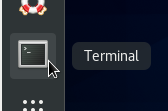
\includegraphics{linuxreader-img021.png}
	\label{fig:DashTerminal}
	\caption{Terminal op de Dash}
\end{figure}


\section{De prompt}
Als je op de command line bent heb je een commandprompt. De commandprompt is het deel voor de cursor, zie \ref{fig:console}

\begin{figure}[h]
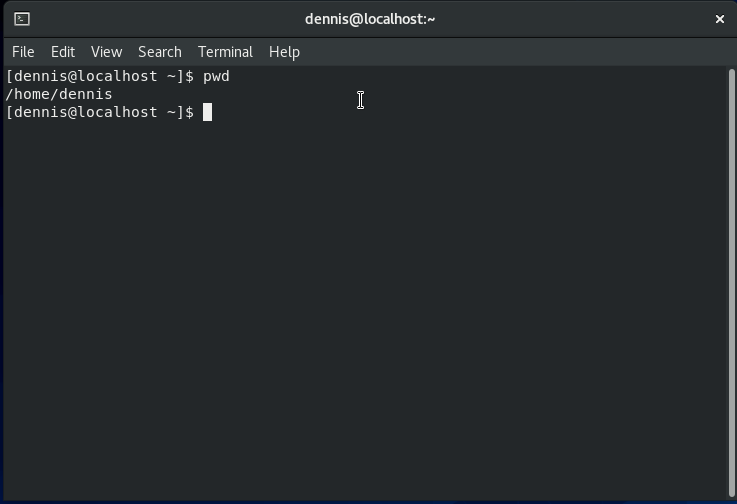
\includegraphics[width=0.8\linewidth]{linuxreader-img022.png}
	\label{fig:console}
	\caption{Console}
\end{figure}

Links staat de login naam, dennis, daarnaast op welke host je bent in gelogd, localhost, daarna volgt de directory
waarin je je nu bevindt, \~{}, en tot slot de prompt voor een normale gebruiker: \$. Als je ingelogt bent als root dan staat er inplaats van een \$ een \#. In deze cursus zullen we alle commando's die je in moet of kan typen op de prompt vooraf laten gaan door een \$ als je het commando als gewone gebruiker moet intypen en door een \# als je het als root moet doen. De \$ en \# moet je dus niet intypen.

Typen we
\begin{lstlisting}[language=bash]
$ pwd
\end{lstlisting}
dan zien we het pad naar de directory waarin we ons bevinden. In dit geval zal dat onze gebruikers
directory zijn met als volledig pad /home/{\textless}gebruikersnaam{\textgreater}. Voor het voorbeeld waarbij de
gebruiker dennis ingelogd is is dat dus /home/dennis. Merk op dat op Linux de directories gescheiden worden door de
forward-slash, /, dit in tegenstelling tot Windows waar de backward-slash, {\textbackslash}, gebruikt wordt als
scheidingsteken.

Nu weten we waar we zijn. Als we willen weten onder welke naam we zijn ingelogd dan gebruiken we
\begin{lstlisting}[language=bash]
$ whoami
\end{lstlisting}
Als je dit commando nu intypt dan zal je je eigen loginnaam zien.

\begin{lstlisting}[language=bash]
$ hostname
\end{lstlisting}
laat zien op welke machine we zitten. Als ik dit commando intyp krijg ik terug `localhost.localdomain', wat
betekent dat mijn machine nog geen echte naam gekregen heeft. Dit kan op je eigen netwerk anders zijn, omdat dit
afhankelijk is van server die de IP-adressen uitdeelt.

\begin{lstlisting}[language=bash]
$ hostname -s
\end{lstlisting}
Geeft alleen de naam van de hostname terug. De -s staat voor short, ofwel kort.

Nu weet je een beetje wie je bent en waar je je bevindt, zowel op welke machine als in welke directory. Welkom thuis.


\section{De shell}
Alles wat je op de prompt intypt wordt opgevangen door de shell. De shell is een schil rond de kernel die commando's van
gebruikers aanneemt en deze doorgeeft naar de kernel. Shell is het Engelse woord voor schelp en eem schelp zorgt ervoor
dat het weekdier dat in de schelp leeft beschermt wordt tegen de buitenwereld. Dat is bij de shell net zo, de shell
beschermt de kernel tegen de gebruiker. De shell wordt ook wel een command interpreter genoemt omdat hij commando's van
de gebruiker interpreteert.

Linux gebruikt standaard de bash shell. Bijna elke linux distributie levert deze mee en heeft deze als standaard shell.
Van oudsher werd op Unix systemen sh meegeleverd. Het was een van de eerste programma's die werd geschreven voor Unix
door Ken Thompson. Tussen 1976 en 1979 schreef Stephen Bourne een vervanging voor sh wat de standaard werd in Version 7
Unix. De naam bleef echter sh op het Unix systeem. Toen het GNU project een vrij en open source systeem wilde maken was
ook daar een van de eerste programma's die er moest komen een shell. Dat werd bash, de naam bash staat voor Bourne
Again SHell. Het is een open source versie van de shell geschreven door Stephen Bourne.

Unix en Linux commando's en bestandsnamen zijn case sensitive. Dat betekent dat `hello.txt' niet hetzelfde is als
`Hello.txt'. Dit zijn twee verschillende bestanden.

Commando's of opdrachten aan de shell hebben een vaste vorm (syntax). Ze zien er zo uit:

\begin{lstlisting}[language=bash]
commando<spatie>optie(s)<spatie>argument(en)
\end{lstlisting}

De spaties zorgen ervoor dat de shell weet wanneer een volgend deel begint, voor de eerste spatie staat het commando,
daarna volgen er geen of enkele opties en tot slot zijn er geen of enkele argumenten. Bijna alle commando's houden deze
syntax aan, hoewel er natuurlijk uitzonderingen zijn.

Het commando ls laat een lijst met bestanden zien. Als we het gebruiken zonder argumenten dan ziet dat er ongeveer uit als in figuur \ref{fig:lsDir}
\begin{figure}[h]
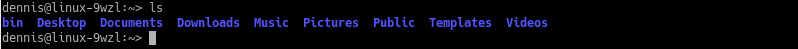
\includegraphics[width=0.9\linewidth]{linuxreader-img023.png}
\label{fig:lsDir}
	\caption{Directory listing}
\end{figure}

Opties worden van argumenten onderscheiden doordat opties beginnen met een min-teken (-). Geven we aan ls een optie me,
bijvoorbeeld -r voor reverse, of wel sorteer omgekeerd dan zien we wat we in figuur \ref{fig:lsRevDir} zien.
\begin{figure}

\includegraphics[width=0.9\linewidth]{linuxreader-img024.png}
	\label{fig:lsRevDir}
	\caption{Reverse order listing}
\end{figure}
We zien nu dat Videos vooraan staat en bin achteraan.

We kunnen ook meerdere opties meegeven. De optie -l geeft een long
list, ofwel een lijst die veel meer informatie per bestand of directory laat zien.
\begin{figure}[h]
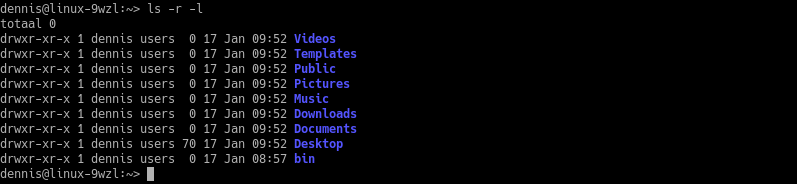
\includegraphics[width=0.9\linewidth]{linuxreader-img025.png}
	\label{fig:lslDir}
	\caption{Reverse and long listing}
\end{figure}
Je mag de opties apart meegeven
zoals we in figuur \ref{fig:lslDir} gedaan hebben maar je mag ze ook samenvoegen zoals:

\begin{lstlisting}[language=bash]
$ ls -lr
\end{lstlisting}
of
\begin{lstlisting}[language=bash]
$ ls -rl
\end{lstlisting}

We kunnen ook een argument meegeven, bijvoorbeeld:
\begin{lstlisting}[language=bash]
$ ls Documents/
\end{lstlisting}
Het argument is de naam van een directory, in dit geval Documents, en we krijgen geen output omdat de directory leeg
is.

De linux shell heeft ook een handigheidje om het leven makkelijker te maken, of beter om minder te hoeven typen, dat
handigheidje heet automatisch aanvullen. Als je op de prompt een p typt zonder een enter te geven en daarna de
tab-toetst indrukt dan gebeurd er niets, druk je nog een keer op de tab-toets dan krijg je de melding:

\begin{lstlisting}[language=bash]
Display all 177 possibilities (y or n)
\end{lstlisting}

Type n want we willen niet 177 mogelijkheden zien. Wat het systeem ons verteld heeft is dat het 177 commando's kent die
met een p beginnen, voegen we nu aan onze p een w toe en typen we 1x tab. Dan vult de shell dit aan met de d en staat
er pwd.

Dit automatische aanvullen kun je doen met commando's maar ook met bestanden en directories. Er wordt weleens gezegd dat
je het toetsenbord van een Linux systeembeheerder kan herkennen aan de versleten tab-toets.


\subsection{History}
Een ander handigheidje van de shell is dat hij een geschiedenis (history) opslaat van gebruikte commando's. Met de
pijltjes toetsen $\uparrow $ (pijltje-omhoog) en $\downarrow $ (pijltje-omlaag) kan je door de geschiedenis van je
commando's scrollen. Omhoog is terug in de tijd en omlaag is het omgekeerde. Met CTRL-c breek je af waar je gebleven
bent en met enter voer je het commando uit.

Met CTRL-r kan je zoeken in je history. Type maar eens CTRL-r en dan de p. Er zal vrijwel direct pwd verschijnen. Op
enter drukken is dan het enige dat nog nodig is om het commando uit te voeren. Als je toch besluit dat je het commando
niet wil uitvoeren dan druk je op CTRL-c om de zoekfunctie te verlaten.

Met !! herhaal je het laatste commando dat je gedaan hebt en met !<commando> herhaal je het
laatste <commando> dat je gedaan hebt. Type nu eens

\begin{lstlisting}[language=bash]
$ !!
\end{lstlisting}

dan zal het pwd commando opnieuw uitgevoerd worden.

\begin{lstlisting}[language=bash]
$ !hostname
\end{lstlisting}
zal de hostname -s uitvoeren want dat is het laatste hostname commando dat we gedaan hebben.

\section{De home-directory}
Wat waarschijnlijk wat uitleg behoeft is dat je prompt laat zien dat je je in de directory \~{} bevindt. Dat is geen
werkelijk bestaande directory maar een handige afkorting die we binnen de CLI kunnen gebruiken om de home-directory van
een gebruiker aan te duiden. Je eigen plek waar je je bestanden kan opslaan heet je home-directory en die kan dus ook
aangeduid worden met de \~{} (tilde). Je bevindt je dus in je eigen home-directory.

De werkelijke plek waar je je nu bevindt in het bestandssysteem kan je laten zien door
\begin{lstlisting}[language=bash]
$ pwd
\end{lstlisting}
te typen. Het pwd\index{pwd} commando toont de werk-directory en pwd staat dan ook voor print working directory. Je zult zien dat
pwd iets terug geeft als
\begin{lstlisting}[language=bash]
/home/dennis
\end{lstlisting}
waarbij `dennis' vervangen is door je eigen gebruikersnaam. De / (forward slash) is het scheidingsteken dat in Linux
gebruikt wordt om directory namen van elkaar te scheiden. Je bevindt je dus drie directories diep vanaf de root van het
bestandssysteem. / is de root-directory, home/ is de tweede directory en dennis/ is de derde directory.

Laten we eens kijken wat er in onze directory te vinden is. Om een overzicht te krijgen van de directories en bestanden
in onze directory typen we `ls'. `ls' is een afkorting voor list. Ofwel geef een lijst van aanwezige files en
directories. Afhankelijk van de distributie of de systeembeheerder zullen er al wat zaken aanwezig zijn. We gaan er
verder vanuit dat je een standaard CentOS installatie hebt gedaan zoals beschreven in een vorige hoofdstuk.

We gaan onze eerste eigen directory aanmaken. Type hiervoor:
\begin{lstlisting}[language=bash]
$ mkdir LinuxCursus
\end{lstlisting}
met behulp van `ls' kan je zien dat er een nieuwe directory bijgekomen is.

Met `cd', change directory, kunnen we ons verplaatsen in de directory:
\begin{lstlisting}[language=bash]
$ cd LinuxCursus
\end{lstlisting}
na de enter zal je zien dat de prompt gewijzigd is en een `ls' geeft een lege output omdat er
niets in de directory staat. Met `pwd' kan je controleren dat je daadwerkelijk in de nieuwe directory staat.

\begin{figure}
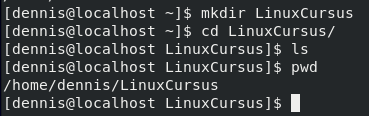
\includegraphics[width=3.8437in,height=1.2083in]{linuxreader-img027.png}
	\label{fig:CreateDirLinuxCursus}
	\caption{Het maken van de LinuxCursus directory}
\end{figure}

Nu gaan we een aantal directories tegelijk aanmaken hiervoor typen we:
\begin{lstlisting}[language=bash]
$ mkdir Data Documenten Muziek
\end{lstlisting}
na een `ls' zie je nu drie nieuwe directories. Zo zie je dat je door meerdere argumenten mee te
geven aan mkdir meer dan 1 directory kan aanmaken.

Met rmdir kan je directories weggooien.
\begin{lstlisting}[language=bash]
$ rmdir Data
\end{lstlisting}
Dit gooit de Data directory weg, na `ls' zie je nu nog maar twee directories.

Als we het systeem verder willen verkennen dan kunnen we met
\begin{lstlisting}[language=bash]
$ cd \~{}
\end{lstlisting}
ervoor zorgen dat we weer in onze home-directory terecht komen, dat scheelt toch een hoop typen die \~{}. \ Als we nu
\begin{lstlisting}[language=bash]
$ cd ..
\end{lstlisting}
typen dan gaan we terug in de directory boom. We komen in de /home/ directory terecht. De dubbele punten naast elkaar
(..) staan voor de directory die 1 stap lager ligt in de boom. We staan nu in de home/ directory die standaard alle
directories van alle gebruikers bevat, dus als er meer gebruikers op het systeem zouden zijn aangemaakt dan zouden ook
van deze gebruikers de home-directories hier te vinden zijn. Een uitzondering is de home-directory van de
systemadministrator van een Linux systeem. Deze beheerder heet `root' en zijn of haar directory is /root/. Daar komen
we later nog een keer op terug.

Als we weer
\begin{lstlisting}[language=bash]
$ cd ..
\end{lstlisting}
typen dan komen we in de / directory terecht. Lager kunnen we niet gaat op een Linux systeem, we zijn nu bij de
root-directory aangekomen. Let op de verwarring die kan ontstaan tussen de /root/ directory en de / directory beiden
heten de root-directory maar de ene is van de gebruiker root en de ander is van het bestandssysteem.

Met alleen het `cd' commando
\begin{lstlisting}[language=bash]
$ cd
\end{lstlisting}
kom je ook weer terug in je eigen home-directory.

\section{Shell variabelen}
Tot nog toe heb je kennis gemaakt met twee variabelen van de shell. PATH en ?. Er zijn er nog veel meer die standaard beschikbaar zijn. Om er een paar te noemen:
\begin{lstlisting}[language=bash]
$ echo $USER
$ echo $SHELL
$ echo $HOME
$ echo $PWD
\end{lstlisting}
om een complete lijst te krijgen van alle variabelen die in je huidige sessie tot je beschikking staan is er het commando \texttt{env}\index{env}\index{commando!env}.
Als je de waarde van een variabele wil wijzigen gebruik je \texttt{export}\index{export}\index{commando!export}:
\begin{lstlisting}[language=bash]
$ echo $PATH
$ PATH=".:${PATH}"
$ export PATH
$ echo $PATH
\end{lstlisting}
met deze opdracht hebben we de . directory toegevoegd aan de PATH variabele. Als we een commando aanroepen en het komt voor in de directory waar we op dat moment in staan dan zal het dat commando uitvoeren. We hoeven dan niet meer het hele pad of de ./ op te geven.

\subsection{Eigen variabelen}
Het is soms handig om eigen variabelen te gebruiken:

\begin{lstlisting}[language=bash]
$ aap=1
$ echo $aap
\end{lstlisting}

Zoals je ziet gebruiken we bij het toewijzen van een waarde aan een variable (stop 1 in de variabele aap) geen \$-teken voor de variabele. Alleen bij het gebruik van de variabele zetten we er een \$-teken voor.

Variabelen in de shell hebben ook geen type, er bestaat geen integer of een string, dus we kunnen net zo makkelijk
doen:

\begin{lstlisting}[language=bash]
$ aap="Dag aap!"
$ echo $aap
\end{lstlisting}

het is een goede gewoonte om voor eigen variabelen kleine letters of kleine letter gemixed met hoofdletters te gebruiken en dat variabelen met alleen hoofdletters gereserveerd zijn voor de interne variabelen van de shell.



% Requires: ls
% Provides: fhs, ps (short)
\chapter{Het bestandssysteem}
\section{Everything is a file}
In Unix en Unix-achtige operating systems zoals Linux is het basis principe dat alles een bestand (file) is. Dit betekent dat alles binnen het systeem; documenten, directories, harddisks, printers, toetsenborden, maar ook processen weergegeven worden als bestanden. Het voordeel hiervan is dat dezelfde commando's en API's gebruikt kunnen worden voor verschillende onderdelen van het besturingssysteem.

Het filesysteem is een enkele boom van bestanden en directories, zonder onderscheid tussen disks en partities. Zelfs verplaatsbare media zoals USB-sticks en DVDs zijn onderdeel van deze boom als ze 'gemount' zijn. Ook processen (/proc) en de kernel (/sys) is voor een groot deel benaderbaar via het bestandssysteem.

Met \texttt{ls} kan je in bijvoorbeeld \texttt{/proc} kijken en zien welke processen er zijn. Je ziet er nummers staan en die nummers komen overeen met de process nummers zoals ook \texttt{ps} die heeft. Doe maar eens:
\begin{lstlisting}[language=bash]
$ ps aux
\end{lstlisting}
en je ziet in de tweede kolom dezelfde nummers staan als in \texttt{/proc/}. \texttt{ps} is ook het commando om te zien welke processen er op je systeem actief zijn. We zullen \texttt{ps} in een volgend hoofdstuk uitgebreid behandelen.

\subsection{Bestandstypen}
In de eerste kolom van \texttt{ls -l} vinden we de bestandrechten en het geeft tevens aan met welk type bestand we te maken hebben. Naast normale bestanden (zoals tekstbestanden) hebben we op POSIX-compliant systemen ook speciale bestanden zoals directories.

\begin{center}
\begin{tabular}{ | l | l | c | }
\hline
Bestandstype & Beschrijving & mode veld \\
\hline
\hline
 normaal bestand & Documenten, etc. & - \\
\hline
 directory & Directories bevatten geen bestand, maar een overzicht van de bestandsnamen waaraan gekoppeld referenties naar iets wat inodes worden genoemd. De inodes bevatten de daadwerkelijke bestanden en meta-data (eigenaar, groep, permissies, time stamps, etc.). Door deze manier van werken kan een bestand (met meta-data) verschillende namen hebben (hard-link), mits binnen \'e\'en bestandssysteem (partitie of disk). Bij verschillende bestandsnamen kunnen dezelfde inodes vermeldt staan. & d \\
\hline
 Symbolic link & een link naar een bestand die over bestandssystemen heen kan gaan & l \\
\hline
Block device & Een apparaat waar van of waar naar toe data in een random manier gestuurd kan worden. Het hoeft dus niet in de juiste volgorde te zijn. Denk aan harddisks waar eerst sector 2014 en dan sector 5678 geschreven kan worden. & b \\
\hline
Character device & Een apparaat waar data in een stroom van characters naar of naar toe gestuurd kan worden & c \\
\hline
FIFO & Ook bekend als named pipes. Een pipe verbindt het ene proces met het andere proces zodat data van proces 1 naar proces 2 gestuurd kan worden. Dit kan maar \'e\'en kant op. & p \\
\hline
Socket & Verbindt net als FIFO's processen, maar dan op een manier dat er twee weg communicatie mogelijk is. & s \\
\hline
\end{tabular}
\end{center}


\section{FHS - Filesystem Hierarchy Standard}
Net als met de standaardisatie van Unix in een POSIX standaard werden er in het begin op Linux Distributies soms bestanden in verschillende directories neergezet. Dat is voor programma's die op die systemen moeten draaien niet handig. Als de ene distributie /var/db heeft voor het plaatsen van databases en de ander /var/databases dan schept dat verwarring. De oplossing die hiervoor gekomen is is de Filesystem Hierarchy Standard. Deze is beschikbaar op \url{https://refspecs.linuxfoundation.org/fhs.shtml}. Hier gaan we heel globaal in op een aantal belangrijke directories, mocht je alle ins en outs willen weten dan raden we je aan om het document een keer te lezen.

\begin{description}
\item [/] De basis van het bestandssysteem wordt bepaald door de root-directory, zo genoemd omdat de vertakkende directories op een boom structuur lijkt en het Engelse root betekend wortel.

Een ls van \texttt{/} laat ons een aantal verschillende directories zien. Waarvan we er een aantal zullen behandelen.

\item [/home/] bevat de directories waarin gebruikers hun bestanden kunnen zetten. Een uitzondering hierop is de directory waarin de root gebruiker (de baas of administrator van het systeem), zijn bestanden kan opslaan. Die directory is \texttt{/root/}.

\item [/etc/] Deze directory bevat de configuratiebestanden van het systeem. Als je een instelling systemwide wilt wijzigen is dit de plek om te gaan zoeken. De configuratie bestanden voor een gebruiker staan in zijn of haar home-directory.

\item [/boot/] Deze directory bevat bestanden die cruciaal zijn voor het opstarten maar die geen commando zijn. Hier vinden we de kernel en bestanden die behoren bij de bootloader.

\item [/dev/] Omdat op een Linus systeem alles een bestand is vind je in deze directory de bestanden die verwijzen aan devices. Devices worden verder besproken in het hoofdstuk over devices. Dus daar gaan we later nog op in.

\item [/var/] is de directory voor de systeem opslag van variabele data zoals bijvoorbeeld de logbestanden, databases, etc. De log bestanden kan je vinden in \texttt{/var/log/}.

\item [/srv/] bevat de data van de diensten die door het systeem worden aangeboden. Data van web- of ftp-servers kan hier gevonden worden.
\end{description}


% Requires: ls, fhs
% Provides: which
\chapter{Commando's}
Het nu volgende hoofdstuk word je uitgelegd waar de commando's op een Linux systeem staan, hoe je met de PATH variabele het zoeken naar commando's kan be\"invloeden en hoe een commando je laat weten of het goed is gegaan of dat er een fout is opgetreden.
Ook krijg je in dit hoofdstuk te lezen hoe je als root commando's uit kan voeren.

\section{Waar zijn de commando's?}
Toen we eerder de p typten en daarna twee keer op de tab-toets toen zagen we dat we 177 commando's hadden die met een p
begonnen. 177 commando's alleen al met een p dat is veel. Een gemiddeld Linux systeem bevat heel veel commando's en dat
is omdat er in de Unix-wereld twee filosofie\"en zijn die bij elkaar aansluiten de eerste is het \ KISS-principle. KISS
staat voor Keep It Simple, Stupid en is oorspronkelijk afkomstig uit de US Navy. En de tweede is Small is Beautiful en
die is afkomstig uit de Economie\footnote{Small Is Beautiful: A Study of Economics As If People Mattered door E. F.
Schumacher}

Op Linux systemen kom je vele kleine commando's tegen die \'e\'en ding goed doen. Dit heeft een aantal voordelen. Omdat
ze maar \ \'e\'en ding doen is de code simpel en is dus makkelijker te controleren op fouten. Omdat niet iedereen in
elk programma weer dezelfde code hoeft te herhalen maar gebruik kan maken van iemand anders zijn programma is de totale
hoeveelheid code klein, een compleet Linux systeem met webserver kan zonder grafische interface ge\"installeerd worden
op een 8G USB-stick. De laatste reden is dat wij als gebruikers vaak zonder te programmeren al heel complexe dingen met
Linux kunnen doen omdat er al zoveel tools al beschikbaar zijn.

Het nadeel van heel veel kleine programma's is dat je het overzicht snel kwijt kan raken. Een van de simpele programma's
is `ls', dat is een afkorting voor list. Veel commando's in Linux zijn afkortingen. De oorspronkelijke ontwikkeling van
Unix werd gedaan op systemen met toetsenborden die niet zo ergonomisch zijn als de onze. Ze hadden toetsen die je met
enige kracht moest indrukken en na een dag programmeren hadden de programmeurs Ken Thompson en Dennis Ritchie en hun
team vaak zere knokkels door overbelasting. Door commando's zo kort mogelijke namen te geven verminderden ze het aantal
toetsaanslagen. Vandaar de korte commando namen.

Type
\begin{lstlisting}[language=bash]
$ ls
\end{lstlisting}
en je zal een aantal blauwe directories op je scherm zien verschijnen. Als je nu
\begin{lstlisting}[language=bash]
$ ls /usr/bin/
\end{lstlisting}
typt dan verschijnen er allemaal groene commando's op je scherm, of beter ze scrollen van je scherm in twee kolommen,
omdat het er te veel zijn. Het past niet op je scherm. Als we de hele lijst willen zien dan zullen we gebruik moeten
maken van een programma de uitvoer van `ls' opdeelt in pagina's die zoveel regels bevatten dat ze het scherm vullen.
Een programma dat dat doet heet `more'. De kunst is nu om de uitvoer van `ls' te koppelen aan `more' en daarvoor is er
de pipe (|) of de pijp. Het pipe-character koppelt twee commando's aan elkaar:
\begin{lstlisting}[language=bash]
$ ls /usr/bin/ | more
\end{lstlisting}
met de spatie-balk kan je nu pagina voor pagina bekijken en met de letter q verlaat je `more'. Nu is more wel heel
simpel en kan het alleen dat wat je nu gezien hebt. Makkelijker zou het zijn als je omhoog en omlaag door de commando's
kan gaan, en misschien zelfs wel zou kunnen zoeken in zo'n lange lijst. Dat kan ook, daarvoor hebben we de opvolger van
`more' die meer kan en `less' heet want less is more.

\begin{lstlisting}[language=bash]
$ ls /usr/bin/ | less
\end{lstlisting}
Nu kan je met de spatie-balk door de pagina's gaan, met de pijltjes omhoog en omlaag per regel door de lijst gaan, met
PgUp en PgDn per pagina omhoog en omlaag gaan en met / kan je zoeken. Type maar eens als je in `less' zit
\begin{lstlisting}[language=bash]
/firefox
\end{lstlisting}
Zo kom je bij het commando `firefox' uit. Ook hier weer is de q-toets de manier om `less' te verlaten.

We hebben nu gezien dat heel veel commando's terug te vinden zijn in de /usr/bin/ directory. Maar dit is maar \'e\'en
plek waar commando's te vinden zijn. Commando's vind je terug in de (s)bin/ directories. We
gebruiken hier een meervoud omdat ze zich op verschillende plekken kunnen vinden. Je bent in de / directory al de bin
en sbin directories tegen gekomen. sbin is voor de systeembeheerder commando's en bin voor
commando's die ook door de normale gebruiker gebruikt kunnen worden.

Maar een Linux systeem zit iets complexer in elkaar. Je hebt waarschijnlijk ook al de /usr/
directory gezien. In die directory kom je een vergelijkbare structuur tegen als in /. Vaak wordt er gezegd dat
commando's in /bin/ en /sbin/ nodig zijn om het systeem op te starten. Alles ze niet direct nodig zijn voor het
opstarten dan vind je ze in /usr/bin/ en /usr/sbin/. Dat geldt ook voor de libraries in /lib/ en /usr/lib/.

Linux is een open source systeem, dus een systeembeheer kan ook bepalen dat bepaalde software
door hemzelf gecompileerd wordt omdat hij bijvoorbeeld een nieuwere versie beschikbaar wil maken dan door de
distributie geleverd wordt. Deze lokaal gecompileerde software wordt dan ge\"installeerd in /usr/local/. Dus
/usr/local/bin bevat commando's die afkomstig zijn van lokaal gecompileerde software en /usr/local/lib/ de libraries.

En als laatste is er nog de /opt/ directory. /opt/ is voor voorgecompileerde software die niet onderdeel is van de
distributie maar die bijvoorbeeld gecompileerd is door een commerci\"ele leverancier van software.

Om te bepalen welke directories gebruikt worden voor het zoeken naar een commando is er een variabele aanwezig in de
shell waarin we werken en die variabele heeft de logische naam PATH. Type maar eens:
\begin{lstlisting}[language=bash]
$ echo $PATH
\end{lstlisting}
Dit levert een output op die er ongeveer zo uit ziet: /usr/local/bin:/usr/bin:/bin. Voor een gebruiker met dit PATH
wordt er voor een commando eerst gezocht in /usr/local/bin, daarna in /usr/bin en als laatste in /bin/.

Als we willen weten waar een commando vandaan komt, dan kunnen we \texttt{which} gebruiken:
\begin{lstlisting}[language=bash]
$ which ls
\end{lstlisting}

Met het commando su kan je een andere gebruiker worden (switch user). Type eens:
\begin{lstlisting}[language=bash]
$ su -
\end{lstlisting}
geef het root wachtwoord en type
\begin{lstlisting}[language=bash]
# echo $PATH
# exit
\end{lstlisting}
Na het su commando moet je het password van de root gebruiker geven dat je ingesteld hebt tijdens
de installatie. Je zal nu zien dat het PATH van de root gebruiker ook de sbin/ directories bevat. De root gebruiker
heeft dus veel meer commando's tot zijn beschikking dan een normale gebruiker.

\section{Error codes}
Stel dat we een commando hebben uitgevoerd en we krijgen niets terug, hoe weten we dan zeker dat het goed gegaan is? Dat weten we omdat een commando ook een exit{}-code terug geeft. Een exit{}-code van 0 betekend dat alles goed gegaan is en alles boven 0 dat er iets fout gegaan is. De man-page van het programma kan je vaak meer vertellen over welke exit{}-code wat betekent als je er niet uit komt met de beschrijving van de error. Type het volgende
\begin{lstlisting}[language=bash]
$ touch hello.txt
$ cat hello.txt
$ echo $?
$ cat Hello.txt
$ echo $?
\end{lstlisting}
na de eerste \texttt{echo \$?} krijg je een 0 en na de tweede \texttt{echo \$?} een 1. Dat komt omdat het eerste commando uitgevoerd kan worden en het tweede niet. Het bestand Hello.txt (met een hoofdletter) bestaat niet.

Het \$-teken betekent dat we te maken hebben met een variabele. Het vraagteken is een speciale variabele die de shell gereserveerd heeft om de exit-code in op te slaan.


% Requires: fhs
% Provides: man, locate, info, apropos
\chapter{Linux documentatie}
Bijna elk linux-systeem is standaard voorzien van een uitgebreide set van documentatie. De
meeste documentatie bevat de man-pages. `man' is een afkorting voor Manual ofwel handleiding. Dat zal je vaker tegen
gaan komen dat commando's op een Linux en andere Unix-systemen afkortingen zijn. Het afkorten scheelt typen, wat
cruciaal was op de oude stugge toetsenborden van de PDP-systemen waarop Unix is ontworpen. Op deze toetsenborden kreeg
je zere vingers van het typen, dus alles dat typen bespaarde was meegenomen.

\section{man-pages}
\index{Manual pages!man-pages}
De op het systeem aanwezig help van een Unix-achtig systeem is te vinden in de man-pages. De online Manual is verdeeld
in hoofdstukken.

\begin{enumerate}
\item Executable programs or shell commands
\item System calls (functions provided by the kernel)
\item Library calls (functions within program libraries)
\item Special files (usually found in /dev)
\item File formats and conventions eg /etc/passwd
\item Games
\item Miscellaneous (including macro packages and conventions), e.g. man(7), groff(7)
\item System administration commands (usually only for root)
\item Kernel routines [Non standard]
\end{enumerate}

Voor gebruikers zijn de belangrijkste hoofdstukken die over de commando's gaan, 1 en 8, en die over de configuratie
bestanden 5. Om een beetje vertrouwd te raken met de man-pages gaan we de manual page over man bekijken. Type:

\begin{lstlisting}[language=bash]
$ man man
\end{lstlisting}

Met de pijltjes toetsten omhoog en naar beneden kan je door de pagina scrollen en met q verlaat je de manual-pagina.
Scrollend door de pagina kom je ook de hierboven al genoemde hoofdstuk indeling tegen. Verder kom je kopjes tegen met
hoofdletter. Veel voorkomende koppen zijn:

\begin{verbatim}
NAME: naam van het commando met een korte uitleg

SYNOPSIS: syntax van het commando

DESCRIPTION: een beschrijving van het commando

OPTIONS: welke opties kent het commando

EXAMPLES: voorbeelden hoe het commando te gebruiken

AUTHORS: wie heeft de manual-page geschreven

SEE ALSO: doorverwijzingen naar andere documentatie
\end{verbatim}

Om snel te zoeken naar bepaalde stukken in een manual-page kan je de / gebruiken. Als je een man-page open hebt staan en
je typt

\begin{lstlisting}[language=bash]
/EXAMPLES
\end{lstlisting}

en deze kop bestaat in de pagina dan kom je meteen bij de examples terecht. Snel door de man-pages scrollen kan door
gebruik te maken van PgUp en PgDn toetsen.


\section{Waar vind ik iets?}
\begin{figure}

\includegraphics[width=0.4\linewidth]{linuxreader-img028.png}
	\caption{Het zoeken van informatie}
\end{figure}

Om uit te vinden welk commando je kan gebruiken om iets op het systeem te bereiken kan je man -k gebruiken. Een
alternatief commando is apropos. Type eens:

\begin{lstlisting}[language=bash]
$ apropos `make directories'
\end{lstlisting}
je vindt dan het `mkdir' commando. Het nadeel van dit zoek systeem is dat het redelijk specifiek is.

\begin{lstlisting}[language=bash]
$ apropos `make directory'
\end{lstlisting}
doet niets. Als je het dus niet meteen vindt probeer dan enkelvoud- en meervoudsvormen.

Heb je een commando gevonden waarvan je denkt dat het is wat je nodig hebt probeer dan man -f of whatis.

\begin{lstlisting}[language=bash]
$ whatis mkdir
\end{lstlisting}

Dit geeft een korte beschrijving van een commando en voor de volledige manual gebruiken we het man commando:
\begin{lstlisting}[language=bash]
$ man mkdir
\end{lstlisting}

Extra uitleg van een commando kan vaak ook gevonden worden door -h of --help aan het commando toe te voegen met een
spatie.

\begin{figure}[H]
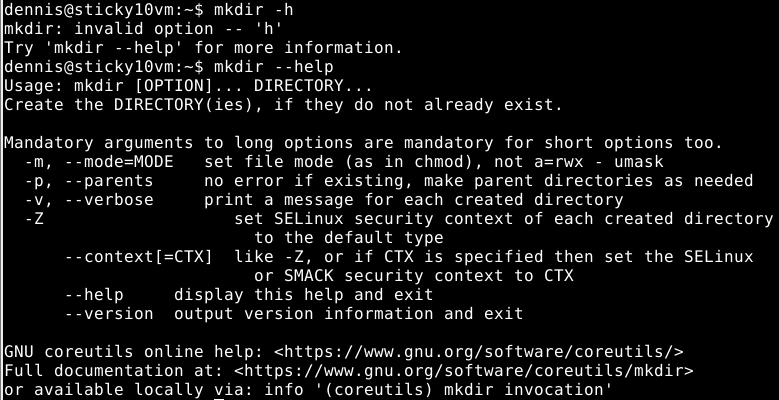
\includegraphics[width=0.8\linewidth]{linuxreader-img029.png}
	\label{fig:DocHelp}
	\caption{Gebruik van -h of --help}
\end{figure}

Zoals je ziet in \ref{fig:DocHelp} dat -h een error melding geeft en ons vertelt dat we -{}-help moeten gebruiken. Ook wordt er verteld wat we de
volledige documentatie online kunnen vinden in de info-documentatie.


\section{Info}
The GNU-project heeft een eigen documentatie systeem ontworpen dat info genoemd wordt. Het is
een hypertext, dus met links, gerelateerd systeem. Dit is dus documentatie dat je naast man tegen komt op systemen.
Mocht je dus in man niet vinden wat je zoekt, misschien kan je dan eens info proberen. Ook in info werken de pijltjes
voor het scrollen en is q er weer om het systeem te verlaten. Een extra functie is de enter-toets die je kan gebruiken
om een link te volgen.

\section{/usr/share/doc}
Een andere plek waar we op ons systeem informatie kunnen vinden is in de /usr/share/doc directory. Met het commando `ls'
kan je een listing van een directory opvragen. Type

\begin{lstlisting}[language=bash]
$ ls /usr/share/doc
\end{lstlisting}

en een enorme lijst van directories vliegt over je scherm. Dit is de documentatie van elk pakket dat op het systeem
ge\"installeerd is. Een linux systeem is opgebouwd uit allerlei software pakketten die vanaf source code door de
distributie maker gecompileerd zijn. De informatie die met de source code meekwam, zoals de licentie-bestanden,
eventuele FAQ-bestanden, READMEs etc. die vind je terug in de subdirectories van /usr/share/doc. Belangrijk zijn vaak
de voorbeeld configuratie-bestanden.

\section{Internet}
Als laatste documentatie bron willen we graag het Internet vermelden. Omdat GNU/Linux een open source besturingssysteem is is er heel veel online te vinden. De kans dat jij als eerste tegen een probleem aanloopt is zeer klein. Het is dus naast de voornoemde bronnen \'e\'en van de eerste zaken om te raadplegen.

De broncode van alle software is openbaar en veel van de projecten hebben hun eigen website met vaak ook een eigen forum\index{forum} om contact te houden met gebruikers. Veel informatie is terug te vinden in de fora en de FAQs\index{FAQ}.



% Requires: fhs
% Provides: touch, cat, mkdir, rmdir, >, >>, <, <<, redirects
\chapter{Werken met bestanden}
Als alles een bestand is in Linux dan is het werken met \index{Bestanden}bestanden het belangrijkste wat er is. Dit hoofdstuk gaat je dan ook de basisbeginselen bijbrengen van het werken met bestanden.

\section{Directories}
Om data op een computer te structureren is het handig om de data te verdelen over directories\index{Directories}. Directories zijn ook bekend als mappen\index{Mappen} en folders\index{Folders}. Wij zullen alleen nog spreken van directories omdat binnen de Unix-wereld de meest gebruikte term is.

Een directory maak je aan met het commando \texttt{mkdir}\index{mkdir}\index{Directories!mkdir}:
\begin{lstlisting}[language=bash]
$ mkdir LinuxCursus
\end{lstlisting}
Met \texttt{ls} kan je controleren of de directory ook daadwerkelijk aangemaakt is.

Je kan ook meerdere directories tegelijk aanmaken door ze als een lijst op te geven, gescheiden door spaties:
\begin{lstlisting}[language=bash]
$ mkdir Aap Noot Mies
\end{lstlisting}

Soms wil je ook een heel pad gelijk aanmaken met:
\begin{lstlisting}[language=bash]
$ mkdir Boom/Roos/Vis/Vuur
\end{lstlisting}
gaat dat niet lukken, want de Boom directory bestaat niet. Gelukkig kan je aan \texttt{mkdir} en optie meegeven die vertelt dat \texttt{mkdir} ook alle onderliggende directories moet aanmaken:
\begin{lstlisting}[language=bash]
$ mkdir -p Boom/Roos/Vis/Vuur
\end{lstlisting}
Gebruik \texttt{ls} om te controleren dat alle directories aanwezig zijn.

Tot slot wil je ook instaat zijn om directories weg te gooien. Met \texttt{rmdir}\index{rmdir}\index{Directories!rmdir} kan dir als de directories leeg zijn.
\begin{lstlisting}[language=bash]
$ rmdir Aap Noot Mies
\end{lstlisting}
gooit keurig alle aangemaakte directies weg. Controleer dit met \texttt{ls}. Maar doen we:
\begin{lstlisting}[language=bash]
$ rmdir Boom
\end{lstlisting}
dan krijgen we een error melding, want de \texttt{Boom} directory is niet leeg. We zullen dus eerst alle andere directories moeten weggooien, te beginnen met \texttt{Vuur}, dan \texttt{Vis}, dan \texttt{Roos} en tot slot kunnen we pas \texttt{Boom} weggooien. Gebruik \texttt{rmdir} om alle directories \textbf{behalve} Boom te verwijderen. De \texttt{Boom} directory moet dus blijven bestaan. 

\section{Bestanden maken en stdin, stdout en stderr}
Zorg dat je in de directory LinuxCursus staat en type:

\begin{lstlisting}[language=bash]
$ touch hello.txt
\end{lstlisting}

Na de Enter lijkt er helemaal niets te gebeuren. Dit is met de meeste Linux commando's het geval. Als het goed gegaan is
dan laten ze niets weten, een beetje als ``geen nieuws, is goed nieuws''. Doen we een `ls' dan zien we dat er een
bestand is aangemaakt dat hello.txt heet.

Met touch kunnen we dus bestanden aanmaken, dit zijn lege bestanden. Type maar eens:

\begin{lstlisting}[language=bash]
$ cat hello.txt
\end{lstlisting}

dan zal je zien dat er weer niets op je scherm verschijnt. En dat is goed! Het `cat' commando plaatst de inhoud van een
bestand op het scherm en daar we een leeg bestand hebben opgevraagd is wat er op het scherm komt dus niets en omdat dat
succesvol is verlopen hoeft cat ook geen foutmelding te laten zien en met de wetenschap dat geen nieuws, goed nieuws is
is cat klaar.

In de acties die we nu hebben doorlopen staat er dat echo tekst naar het scherm schrijft en cat
bestanden op het scherm afbeeldt. Dat is inderdaad wat er gebeurt, maar vanuit het Linux gezien niet helemaal correct.
Zowel echo als cat schrijven naar de standaard output en in de terminal is het scherm de standaard output. De standaard
output wordt vaak afgekort als stdout.

We kunnen de standaard output ook omleiden (redirect) naar bijvoorbeeld een bestand:

\begin{lstlisting}[language=bash]
$ echo 'Ik werk met Linux' > hello.txt
\end{lstlisting}

We zien nu dat de zin die we met echo afbeelden niet meer op het scherm verschijnt. Hij is verdwenen en er lijkt weer
helemaal niets gebeurd te zijn. Als we nu

\begin{lstlisting}[language=bash]
$ cat hello.txt
\end{lstlisting}

doen dan zien we waar onze zin is gebleven. Hij is hello.txt terecht gekomen. We hebben de stdout van echo in hello.txt
gestopt.

Laten we dat nog eens doen:

\begin{lstlisting}[language=bash]
$ echo 'Hello World!' > hello.txt
\end{lstlisting}

Doen we een cat van hello.txt dan zien we dat onze eerste zin verdwenen is en er alleen nog 'Hello World!' in hello.txt
zit. We hebben kennelijk ons bestand overschreven met nieuwe inhoud. We kunnen ook tekst toevoegen aan een bestand:

\begin{lstlisting}[language=bash]
$ cat 'Ik werk met Linux' >> hello.txt
\end{lstlisting}

door gebruik te maken van het dubbele groter dan teken voegen we een regel toe aan het eind van het bestand. De oude
regel zie je met cat als eerste en daaronder komt onze nieuwe regel.

Zou er als we een stdout hebben ook een standaard input zijn en kunnen we daar dan van lezen? Ja, die is er. Als je
typt:

\begin{lstlisting}[language=bash]
$ cat < hello.txt
\end{lstlisting}

dan vertellen we eigenlijk dat cat de invoer (stdin) op het scherm moet afbeelden. Maar ja, dan moeten we een spatie en
een <-teken extra typen en dat doen we liever niet.

Naast de standaard input en standaard output is er ook nog standaard error (stderr), waar de foutmeldingen naartoe gaan.
Laten we eens een fout maken door een niet bestaan bestand aan cat te geven:

\begin{lstlisting}[language=bash]
$ cat Hello.txt
\end{lstlisting}

Je krijgt nu een foutmelding dat Hello.txt niet bestaat. Linux is case-sensitive dus hello.txt is niet hetzelfde als
Hello.txt. De standaard output, input en error zijn genummerd in Linux. Stdin is 0, stdout is 1 en stderr is 2. Nu we
dit weten zouden we het volgende kunnen doen:

\begin{lstlisting}[language=bash]
$ cat Hello.txt 2> Hello_error.txt
\end{lstlisting}

We zien nu geen foutmelding meer op ons scherm en hebben de stderr omgeleid (redirect) naar het bestand
Hello\_error.txt. Doen we nu een
\begin{lstlisting}[language=bash]
$ cat Hello_error.txt
\end{lstlisting}
dan zien we dat de foutmelding daar is opgeslagen.

Deze vormen van het redirecten (omleiden) van data stromen gebeurt in Linux heel vaak. Programma's schrijven
bijvoorbeeld de fouten die ze tegen komen naar een log bestand. Dit doen ze door de stderr te redirecten en de error
regels toe te voegen aan het bestand, bijvoorbeeld 2>>error.log. Als ze dit doen met een
datum- en tijdmelding dan kan je heel makkelijk problemen opzoeken.

Wij hebben nu geleerd om bestanden aan te maken en om invoer en uitvoer te redirecten.


\section{Bestanden kopie\"eren, verplaatsen, hernoemen, verwijderen}
Om bestanden te kopie\"eren gebruiken \texttt{cp}\index{cp}\index{Bestanden!cp} van het Engelse copy:
\begin{lstlisting}[language=bash]
$ cp hello.txt Boom/hello.txt
\end{lstlisting}
We kunnen ook gelijk de naam veranderen als we dat willen:
\begin{lstlisting}[language=bash]
$ cp hello.txt Boom/Hallo.txt
\end{lstlisting}

Om bestanden verplaatsen gebruiken \texttt{mv}\index{mv}\index{Bestanden!mv} van het Engelse move. Het verschil met copy is dat een bestand niet meer op de oorspronkelijke plek terug te vinden is. Bij move heb je dus maar 1 bestand na de handeling, na copy heb je 2 bestanden.
\begin{lstlisting}[language=bash]
$ mv Boom/Hallo.txt .
\end{lstlisting}
Het \texttt{mv} commando kunnen we ook gebruiken om bestanden van naam te veranderen:
\begin{lstlisting}[language=bash]
$ mv Hallo.txt hallo.txt
\end{lstlisting}

Voor het weggooien van bestanden gebruiken we \texttt{rm} van remove.
\begin{lstlisting}[language=bash]
$ rm hallo.txt
\end{lstlisting}

Omdat alles een bestand is op een Linux systeem zijn ook directories bestanden, speciale bestanden, maar toch bestanden. We hebben al gezien dat we met \texttt{rmdir} lege directories weg kunnen gooien. Zouden we nu \texttt{rm} kunnen gebruiken om ook directories weg te gooien. Ja, dat kan, maar ook hier geldt dat de directory leeg moet zijn.
\begin{lstlisting}[language=bash]
$ rm Boom
\end{lstlisting}
geeft weer een foutmelding. Het systeem zegt tegen ons dat \texttt{Boom} een directory is. Als we tegen \texttt{rm} vertellen dat hij de zaken recursive weg met gooien, dan zal de hele boomstructuur wegggegooid worden:
\begin{lstlisting}[language=bash]
$ rm -r Boom
\end{lstlisting}
De \texttt{-r} optie verteld aan rm dat hij vanuit de diepste plek in de Boom directory moet beginnen met bestanden (en directories) weg te gooien net zo lang tot hij de directory Boom weg kan gooien. In ons voorbeeld is het niet veel dat \texttt{rm} te doen heeft, maar je zal niet de eerste zijn die met \texttt{-r} meer weggooid dan de bedoeling was en dat tot de ontdekking komt dat een Linux systeem geen undelete kent. Terug halen van data is er dan ook niet bij.


% Requires: fhs
% Provides: vi, vim, nano, pico
\chapter{Het gebruik van een editor}
Op de commandline heb je geen menu's en vaak geen muis om door een applicatie te navigeren. Het maken van documenten is dan ook een stuk lastiger dan in een grafische interface. Toch zijn er oplossingen om op de commandline te werken met bestanden. Een tekstverwerker\index{tekstverwerker} op de commandline heet een editor\index{editor}. Er zijn verschillende editors bedacht en in gebruik. Een van de oudste voor Unix geschreven editors is \texttt{vi}.

Een van de grote namen achter Unix is Ken Thompson. De eerste drie commando's die hij schreef voor het jonge Unix systeem waren \texttt{as} (assembler), \texttt{ed}\index{ed} (editor) en \texttt{sh} (shell). Dennis M. Ritchie bracht verbeteringen aan op \texttt{ed} en vanaf 1969 tot 1976 bleef dit de editor op een Unix systeem. In 1976 kwamen Billy Joy en Chuck Haley met een nieuwe editor die \texttt{ex}\index{ex} werd genoemd. Voor \texttt{ex} schreef Billy Joy ook een soort interface om er makkelijker mee te kunnen werken en die wrapper om \texttt{ex} noemde hij \texttt{vi}\index{vi} (visual interface\index{visual interface}). Vanaf 1979 werd \texttt{ex} geintergreerd in \texttt{vi} en was er alleen nog \texttt{vi}. Later werd \texttt{vi} onderdeel van de Single Unix Specification en daarmee een editor die op bijna elk Unix systeem aanwezig is en dat is nogsteeds het geval. Op bijna alle beschikbare Unix systemen, van BSD tot Linux en Mac OS X is een vorm van \texttt{vi} aanwezig. Dat is dan ook het voordeel van het aanleren van het werken met \texttt{vi}, ja kan je kennis op verschillende platformen gebruiken.

\section{vi, pico, nano}
De eerste redelijk gebruiksvriendelijke editor op Unix was \texttt{vi}. De \texttt{vi} editor kent twee modi. De eerste modus is de \textquote{edit mode} en de tweede is de \textquote{command mode}. Standaard start \texttt{vi} op in de command mode waarin je commando's kunt geven om bestanden te laden of op te slaan en waarin je functies als knippen en plakken kan uitvoeren. De edit modus is die waarin je tekst invoert. Dit onderscheid maakt het voor beginnende gebruikers \texttt{vi} soms verwarrend.

Naast \texttt{vi} zijn er ook andere editors voor Unix-achtige systemen ontwikkeld. De meeste bekende zijn \texttt{pico}\index{pico} en \texttt{nano}\index{nano}. Pico was de oorspronkelijke editor. Nano is ontwikkled door het GNU-project en is een vervanging van pico omdat pico een licentie had die \textquote{problematisch} was. Dat probleem is inmiddels opgelost, maar nano biedt zoveel extra mogelijkheden dat velen de voorkeur geven aan nano.

Het grote voordeel van nano ten opzichte van vi is zijn gebruiksvriendelijke interface. Nano kent geen edit en command mode zoals vi. Nano gebruikt control codes om commando's te geven en is direct beschikbaar voor de invoer van tekst van de gebruiker.

\section{vim}
De naam \texttt{vim}\index{vim} staat voor Vi IMproved\index{Vi IMproved}. Of wel een verbeterde versie van \texttt{vi}. Bram Molenaar, een Nederlandse software ontwikkelaar, schrijft al sinds 1991 aan de code van \texttt{vim} en zijn verbeteringen zijn zo populair dat op alle Linux systemen alleen nog \texttt{vim} ge\"installeerd wordt. Je kan op een Linux systeem \texttt{vim} opstarten als \texttt{vi} waarmee je zoveel mogelijk de functionaliteiten krijgt als het oude \texttt{vi} en je kan \texttt{vim} opstarten als \texttt{vim} waarmee je alle nieuwe toevoegingen van Bram Molenaar en zijn medeontwikkelaars krijgt.

\texttt{vim} is niet een van de makkelijkste editors maar heeft als grote voordeel, zoals eerder gezegd, dat het beschikbaar is op elk willekeurig Unix systeem.

\subsection{vim opstarten}
Het kan zijn dat \texttt{vim} nog niet geinstalleerd is. Mocht dat het geval zijn, installeer dan \texttt{vim} via de packagemanager voor jouw systeem. Voor Debian systemen is dat:\index{vim!installeren}

\begin{lstlisting}[language=bash]
$ sudo apt-get install vim
\end{lstlisting}

De meeste gebruikelijke manier om \texttt{vim} op te starten is door aan \texttt{vim} meteen een bestandsnaam mee te geven:\index{vim!starten met bestandsnaam}
\begin{lstlisting}[language=bash]
$ vim bestand.txt
\end{lstlisting}
Als je klaar bent met het toevoegen van tekst kan je met \textbf{:wq} afsluiten\index{vim!opslaan en afsluiten}. Dit slaat het document op (w)\index{vim!opslaan} en sluit af (q). Wil je de editor verlaten zonder de gemaakte wijzigingen op te slaan, dan gebruikt je \textbf{:q!}\index{vim!afsluiten zonder opslaan}. Het doet een quit (q) zonder verdere vragen stellen.

Een andere manier om vim op te starten is door geen bestandsnaam mee te geven:\index{vim!starten zonder bestandsnaam}
\begin{lstlisting}[language=bash]
$ vim
\end{lstlisting}
de editor weet nu niet onder welke bestandsnaam een bestand opgeslagen moet worden. Bij de write (w) moet je nu dus de bestandsnaam meegeven: \textbf{:w bestand.txt}\index{vim!bestand schrijven} slaat het bestand dat je gemaakt hebt op als bestand.txt. Na deze opdracht kan je met \textbf{:q} vim afsluiten.

Om tekst toe te voegen of te wijzigigen in \texttt{vi} moet je vanuit de command mode\index{command mode} naar de edit mode\index{edit mode} gaan. Hiervoor zijn verschillende commando's beschikbaar. De meest gebruikte zijn \textbf{i} van insert\index{vim!insert} of \textbf{a} van add\index{vim!add}. Om de edit mode\index{edit mode!verlaten} te verlaten gebruik je de \textsc{ESC} toets.

Met het gebruik van het \textbf{i} commando voeg je tekst in v\'o\'or de plek van de cursor. Door gebruik te maken van \textbf{a} voeg je tekst in na de positie van de cursor.

Vanuit de command modus kan je het character waarop je staat verwijderen door gebruik te maken van het \textbf{x} commando, eigenlijk is dit het knippen commando, maar kan gebruikt worden om snel wat characters te verwijderen. Het \textbf{D} commando verwijdert de text vanaf de plek waarop je staat tot het einde van de regel. Het einde van de regel is tot de plek waar je \textsc{ENTER} gegeven hebt, dus niet tot het einde van de regel op het scherm.

Het verwijderen van een complete regel van begin tot eind doe je met \textbf{dd}. Dit commando kan je uitbreiden met aantallen regels door tussen de d's een getal op te geven. Bijvoorbeeld \textbf{d2d} verwijdert 2 regels vanaf de plek waar je staat. En zo kan je ook met \textbf{dl} letters verwijderen. De combinatie \textbf{d5l} verwijdert vanaf de positie van de cursor 5 characters. Om hele woorden weg te gooien gebruik je \textbf{dw} en ook daar geldt de mogelijkheid om meerdere woorden in \'e\'en keer weg te gooiden met \textbf{d3w} gooi je 3 woorden achter elkaar weg.

Met het \textbf{x} commando kan je \'e\'en enkel character knippen.

De traditionele manier om een kopie van een stuk tekst te maken is het gebruik van het \textbf{y} commando\index{vim!copy}. Het \textbf{yl} commando kopieert een character, \textbf{yw} kopieert een woord en \textbf{yy} kopieert regels.

Het \textbf{p}\index{vim!paste} commando kan gebruikt worden om text te plakken. Het \textbf{p} commando is plakken achter de positie van de cursor en \textbf{P} is plakken voor de positie van de cursor.

Een speciale functie van vim en niet van vi is het gebruik van \textbf{v} om een visuele selectie\index{vim!visual selection} maken, met de pijltjes toetsen kan je nu bepalen hoe groot de selectie worden moet. Het commando \textbf{v} geeft je de mogelijkheid om de selectie op character niveau te maken. Met \textbf{V} maak je selecties per regel, hier gebruik je de omhoog en omlaag pijltjes toetsen om je selectie groter of kleiner te maken. Als je de selectie gemaakt hebt gebruik je \textbf{y} om te kopie\"eren of \textbf{d} om het stuk te verwijderen.

Met \textbf{u} kan je een wijziging ongedaan maken.


Met de pijltjes toetsen kun je in de edit mode bewegen door een bestand. De pijltjes links en rechts bewegen de cursor een character per keer naar links of rechts, de op en neer pijltjes bewegen de cursor een regel op en neer.

In de command mode kan je met \textbf{\^} bewegen naar het begin van een regel en met \textbf{\$} naar het einde van de regel. Een grotere sprong is met \textbf{gg} naar het begin van een document en met \textbf{G} naar het einde van het document.

Met \textbf{w} spring je een woord vooruit.

Je kan ook springen naar een bepaalde regel. Hiervoor gebruik je bijvoorbeeld :10. Dit commando sprint naar regel 10 van boven.

Met zoek opdrachten kan je ook door een document bewegen. Het \textbf{/} teken geeft het begin van een zoekopdracht aan. Dit werkt alleen in de command-modus. Met \textbf{/zoeken} zoek je naar het woord zoeken in de tekst. Met de letter \textbf{n} kan je naar het volgende zoekresultaat springen en met \textbf{N} naar het voorgaande.


% Requires: fhs, editor
% Provides: grep, find, globbing, regular expressions, sed
\chapter{Zoeken en vinden}\label{zoekenenvinden}
In dit hoofdstuk ga je leren hoe je op een Linux systeem naar bestanden kan zoeken. Ook ga je leren hoe je in bestanden kan zoeken naar patronen, waarbij woorden patronen kunnen zijn, maar er kan veel meer. Dat alles komt in dit hoofdstuk aan bod.

Om de opdrachten uit dit hoofdstuk te kunnen maken is het van belang om de volgende commando's uit te voeren:
\lstinputlisting[language=bash]{bash/ZoekenVinden.sh}
\lstinputlisting[language=bash]{bash/ZoekenGrep.sh}

\section{Globbing}
Globbing is het gebruiken van wildcards. Wildcards zijn bijvoorbeeld de asterisk (*) en het vraagteken (?). Een asterisk staat voor geen of meer characters en een vraagteken staat voor \'{e}\'{e}n character. Zo kunnen we ontbrekende characters invullen of aanvullen als we niet meer helemaal zeker weten hoe een bestand heet. Stel dat we weten dat we een document gemaakt hebben met de naam \texttt{Plaatje} maar dat we niet meer weten of dat een jpg, png of gif plaatje is. Dan kunnen we een overzicht van alle bestanden in een directory opvragen met:
\begin{lstlisting}[language=bash]
$ ls Plaatje.*
\end{lstlisting}
We krijgen dan de bestanden met een willekeurige extensie terug.

Globbing is een functie die door de shell wordt uitgevoerd. De shell vervangt dus eerst de wildcards door wat er op het bestandssysteem staat en voert dat uiteindelijk aan \texttt{ls}. Als je quotes om het argument zet dan gaat \texttt{ls} opzoek naar een bestand dat \verb|Plaatje.*| heet. Er verschijnt dan keurig de melding dat dat bestand niet bestaat.

Zo kunnen we ook zoeken op de bestandsnamen waarvan we niet meer zeker weten of we het met een hoofdletter of kleine letter hebben geschreven door gebruikt te maken van het vraagteken:
\begin{lstlisting}[language=bash]
$ ls ?laatje.*
\end{lstlisting}

Het toeval wil dat we ooit het recept van een vriend hebben opgeschreven over hoe we huzarensalade moeten maken dus kregen we van het laatste commando terug:
\begin{lstlisting}[language=bash]
plaatje.jpg  Plaatje.png Slaatje.txt
\end{lstlisting}

Als we alleen de bestandsnamen die echt het plaatje bevatten willen vinden dan zullen we gebruik moeten maken van een ander optie die de shell ons biedt, namelijk de blokhaken (\big[\big]). In shell-globbing betekenen de blokhaken een reeks. Een reeks kan zijn \big[1234567890\big], of \big[abcdefg\big], wat trouwens simpeler geschreven kan worden als \big[0-9\big] en \big[a-g\big], maar een reeks mag ook zo simpel zijn als \big[pP\big], dus de hoofdletter P en de kleine letter p.
\begin{lstlisting}[language=bash]
$ ls [Pp]laatje.*
\end{lstlisting}
en zo krijgen we precies terug wat we willen.

Reeksen in globbing zijn heel handig. Je kan bijvoorbeeld een reeks maken [a-zA-Z0-9] zodat je 3 reeksen combineert en zo alles hebt dat geen leesteken bevat. Als je ook bestandsnamen hebt die een spatie kan bevatten maak je er \big[\textbackslash~a-zA-Z-0-9\big] van. Let op het escape (\textbackslash) character voor de spatie. Zonder dat character zou de shell aan ls twee argumenten meegeven, want er staat een spatie en spaties (white-space) scheiden argumenten. Dus ls krijgt de opdracht om een list te doen van '\big[' en van 'a-zA-Z0-9\big]' en dat is niet wat we willen. We willen dat onze reeks \'{e}\'{e}n argument is, vandaar dat we de spatie ''escapen'' zoals dat heet. Door het escape-character behandeld de shell de spatie niet als scheidingsteken van argumenten maar als onderdeel van de reeks.

\section{Zoeken naar bestand}
Om op de commandline bestanden te zoeken die ergens op het filesysteem staan is er het commando \texttt{find}. De syntax van het \texttt{find} commando ziet er ongeveer zo uit:
\begin{lstlisting}[language=bash]
find <path> <options> <action>
\end{lstlisting}
\texttt{find} zoekt vanaf het opgegeven \texttt{path} naar bestanden die voldoen aan de opgegeven opties en voert daar de opgegeven \texttt{action} op uit. De standaard actie is om de naam van het bestand inclusief het complete pad te printen naar de standaard output. De zoekactie van \texttt{find} is als je dat niet limiteert recursief en dus door alle subdirectories. Dat betekent ook dat als je / als pad op geeft dat het hele bestandssysteem doorzocht wordt (dat kan even duren).

Met zo'n grote boom van directories is het van belang dat je op een simpele manier bestanden terug kan vinden. Om te
zoeken naar bestanden of directories is er het commando `find'. De syntax van `find' ziet er zo uit:

\begin{lstlisting}[language=bash]
$ find \ [-H] \ [-L] [-P] [-D debugopts] [-Olevel] [starting-point...] [expression]
\end{lstlisting}

Dit is geknipt en geplakt uit de man-page waar je uitgebreide documentatie kan vinden over find. Om een idee te krijgen
hoe find werkt type:

\begin{lstlisting}[language=bash]
$ find \~{} -name ``Muziek'' -print
\end{lstlisting}

Bij mij op het systeem was het antwoord
\begin{lstlisting}[language=bash]
/home/dennis/LinuxCursus/Muziek
\end{lstlisting}

Bij jou is dennis natuurlijk weer vervangen door je eigen gebruikersnaam. Print is de standaard functie van find, en
daarom vonden de programmeurs van find dat als je geen opdracht meegeeft dat find dan ook print doet. Dus korter kan
het zo
\begin{lstlisting}[language=bash]
$ find \~{} -name ``Muziek''
\end{lstlisting}

Die \~{} is makkelijk als je in je home-directory wilt zoeken, maar wat als je in bijvoorbeeld /etc/ staat en in die
directory wilt zoeken? Daar is ook over nagedacht. We hebben al `..' gezien als een aanduiding voor een lager gelegen
directory, maar zo is er ook de `.' als we `deze'-directory bedoel. En met deze bedoelen we de directory waarin we nu
staan. Dus we kunnen ook het volgende doen:

\begin{lstlisting}[language=bash]
$ find . -name ``Muziek''
\end{lstlisting}

En voor wie niets tegen typen heeft mag je natuurlijk ook de hele directory opgeven
\begin{lstlisting}[language=bash]
$ find /home/dennis/ -name ``Muziek''
\end{lstlisting}

Met -name geven we op dat we naar een bestandsnaam zoeken en een bestandsnaam kan ook een directory zijn. Als we
onderscheidt willen maken tussen bestanden en directories kan kunnen we een -type meegeven:
\begin{lstlisting}[language=bash]
$ find . -type d -name ``Muziek''
\end{lstlisting}

Zal dezelfde output geven want type d is een directory, maar als doen
\begin{lstlisting}[language=bash]
$ find . -type f -name ``Muziek''
\end{lstlisting}

dan vinden we niets, want het type f is een regulier bestand en Muziek is een directory.

Om dat te testen doen we het volgende
\begin{lstlisting}[language=bash]
$ touch \~{}/LinuxCursus/Documenten/leeg\_bestand.txt
$ find . -type f -name ``leeg\_bestand.txt''
\end{lstlisting}

Met touch kan je een nieuw leeg bestand aanmaken en dat hebben we gedaan en daarna hebben we find naar dat nieuwe
bestand laten zoeken. Nou lijkt dit een wat onzinnige actie omdat we al weten waar het bestand is, maar het geeft ons
een optie om een andere functie van find te demonstreren, namelijk het zoeken naar lege bestanden op het systeem:
\begin{lstlisting}[language=bash]
$ find . -size 0
\end{lstlisting}
de -size optie geldt alleen voor bestanden, de -empty optie laat naast lege bestanden ook lege directories zien
\begin{lstlisting}[language=bash]
$ find . -empty
\end{lstlisting}

Het find commando kent nog veel meer opties zoals zoeken naar de datum en tijd waarop een bestand is aangemaakt of een
moment later of eerder dan een bepaalde datum en tijd. De man-page van find documenteert al deze verschillende opties
en op Internet is heel veel uitleg te vinden hoe je find met al deze opties kan gebruiken. Een laatste functie van find
willen je nog meegeven. De kan behalve met -print find ook andere dingen laten doen dan de gevonden elementen printen,
je kan find ook vertellen om een actie uit te voeren, zoals het deleten van de gevonden elementen:

\begin{lstlisting}[language=bash]
$ find . -size 0 -delete
\end{lstlisting}
een ls van LinuxCursus/Documenten/ zal laten zien dat het bestand leeg\_bestand.txt niet meer bestaat. Pas wel op, dit
kan gevaarlijke situaties opleveren.

\begin{lstlisting}[language=bash]
$ find LinuxCursus/ -empty -delete
\end{lstlisting}

Dit commando zoekt in de LinuxCursus naar alle directories en bestanden die leeg zijn. Bestanden
hadden we niet meer, maar er stonden nog wel twee directories in (Documenten en Muziek), beide directories waren leeg
en werden door find dan ook keurig verwijderd van het systeem. Toen kwam find nog de directory LinuxCursus tegen, en ja
die was inmiddels ook leeg, dus heeft find die ook weggegooid!

\section{Zoeken in bestanden}

Soms zou je willen dat je in een bestand kunt zoeken. Natuurlijk kan je met in een tekstverwerker of een editor zoeken in een bestand, maar wat nu als je niet zeker meer weet in welk bestand het was dat je iets geschreven had. Dat kan zomaar gebeuren als je een boek zoals dit aan het schrijven bent. Dit boek is opgebouwd uit allemaal kleine bestanden die te samen het boek vormen. Op deze manier hou ik de onderwerpen gescheiden en hoef ik niet elke keer te scrollen om bij een ander deel te komen. Ik kan ook twee onderwerpen in twee verschillende terminals te gelijk open hebben staan en zo parallel aan de stukken werken. Dit deel gaat over hoe we in bestanden kunnen zoeken zonder dat we een tekstverwerker hoeven te gebruiken.

Er zijn verschillende commando's die we kunnen gebruiken, de meest gebruikte is denk ik \texttt{grep}. Met \texttt{grep} kan je door regular expressions te gebruiken zoeken in bestanden. Meer over regular expressions vind je in de volgende sectie. Nu gaan we vooral kijken naar hoe het \texttt{grep} commando werkt.



\texttt{grep} is de Global Regular Expression Parser\index{grep}\index{commando!grep}\index{Global Regular Expression Parser}. De naam \texttt{grep} vindt zijn oorsprong in een zoekopdracht uit \texttt{ed}, een editor: \texttt{g/re/p} wat stond voor zoek door de hele tekst (\textbf{g}lobal) naar deze \textbf{r}egular \textbf{e}xpression en druk deze af (\textbf{p}rint). \texttt{re} werd dan vervangen door een regular expression.

Om te zien hoe \texttt{grep} werkt gaan we eerst een paar bestanden met inhoud aanmaken.

\lstinputlisting[language=bash]{bash/ZoekenGrep.sh}

\section{Regular Expressions}
Regular expressions\index{regular expressions} zijn speciale karakters waarmee je makkelijker in complexe data-sets kan zoeken. De naam regular expression wordt vaak afgekort tot regexp\index{regexp} of regex\index{regex}.

Regular expressions zoeken regels waarin een bepaalde een bepaalde reeks aan karakters voorkomt en beeldt dan de gehele regel af. Je kan zoeken in bestanden of in de output van een commando.

De basis van regular expressions is een aantal karakters met een speciale betekenis:

\begin{tabular}{| l | l |}
\hline
. & Is een willekeurig karakter \\
\hline
? & Is exact 1 karakter \\
\hline
* & Herhaal de voorgaande expressie 0 of meer keren \\
\hline
$\textasciicircum$ & Begin van de regel \\
\hline
\$ & Einde van de regel \\
\hline
$\backslash$ & Zorg ervoor dat speciale karakters als echte karakters behandeld worden \\
\hline
\{\} & Zorg dat dat een regular expression een eenheid (groep) vormt \\
\hline
\end{tabular}

Deze speciale karakters kunnen we gebruiken om regular expressions te maken. We beginnen met de . en het ?:
\begin{lstlisting}[language=bash]
$ mkdir regex
$ cd regex
$ touch aap.txt
$ touch ap.txt
$ touch pa
$ touch filetxt
$ ls | grep a?*p
$ ls | grep a.*p
\end{lstlisting}
merk op dat het verschil in output van de twee \texttt{ls} commando's zit in het aantal keren dat een letter voor moet komen. ?* zegt dat er 1 of meer karacters moeten zijn, terwijl .* zegt dat het 0 of meer karakters moet zijn.

\begin{lstlisting}[language=bash]
$ ls | grep $\textasciicircum$a
$ ls | grep a$
\end{lstlisting}
Met het $\textasciicircum$ zoeken we vanaf het begin van de regel, dus de regel moet beginnen met een a. Met de \$ zoeken we vanaf het einde, dus de regel moet eindigen met een a.

Als we willen bestanden willen zien die op .txt eindigen dan willen dat de punt onderdeel is van onze zoek opdracht en willen we niet dat de punt gezien wordt als een willekeurig karakter. Vergelijk de volgende twee commando's en hun uitkomst:
\begin{lstlisting}[language=bash]
$ ls | grep '.txt'
$ ls | grep '\.txt'
\end{lstlisting}

Let op de ticks om de regular expression. De ticks zorgen ervoor dat de regular expression bij \texttt{grep} terecht komt en niet al door de shell wordt uitgevoerd. De shell is natuurlijk de eerste die de complete commando regel krijgt. Het is de shell die moet beslissen wie welk deel uitvoert. Voor \texttt{ls} is dat niet zo moeilijk  daar wordt de opdracht aan \texttt{ls} overgelaten, maar voor de regular expression bij \texttt{grep} ontstaan er twee mogelijkheden. De shell lost zelf al een deel van de regular expression op en geeft wat er over blijft aan grep of de shell geeft de complete regular expression aan grep. Dat laatste is wat we in dit geval willen. Vergelijk met je hiervoor gekregen uitkomsten eens met:
\begin{lstlisting}[language=bash]
$ ls | grep \.txt
\end{lstlisting}
Wat hopelijk opvalt is dat ondanks de $\backslash$ er niet gefilterd wordt op .txt maar op alles dat een willekeurig karakter heeft met daarachter txt. Dat komt omdat de shell de $\backslash$. al matched met de output van \texttt{ls}. Dit is dus wel iets om op te letten met regular expressions. Het is altijd veilig om de regex tussen ticks te zetten. Dan weet je zeker dat de regex bij grep uitkomt en niet bij de shell.

Soms willen we kunnen aangeven hoe vaak een bepaald karakter achter elkaar voorkomt. Daarvoor hebben we de curly braces (accolades).
\begin{lstlisting}[language=bash]
$ ls | grep -E 'a{2}'
\end{lstlisting}
Zoek zelf in de man-page van grep op wat -E betekent.

\section{Zoek en vervang}
We kunnen ook regels zoeken in een bestand die aan een bepaald patroon (regex) voldoen en dan het patroon vervangen door iets anders. Een van de meest gebruikte tools daarvoor heet \texttt{sed}\index{sed}.

\begin{lstlisting}[language=bash]
$ ls -1
$ ls | sed -e 's/aap/noot/'
\end{lstlisting}
overal waar aap stond staat nu noot. Op de disk is er niets gewijzigd, we hebben alleen de output van ls aangepast.

Om iets meer van \texttt{sed} te leren gaan we eerst een bestand aanmaken:
\lstinputlisting[language=bash]{data/stageverslag.txt}

Hier zitten wat taal fouten in. Die gaan we zoeken en ook vervangen. We beginnen met het gebruik van Me aan het begin van de eerste twee alinea's. Dat moet natuurlijk Mijn zij.
\begin{lstlisting}[language=bash]
$ sed -e 's/^Me/Mijn/'
\end{lstlisting}
Op het scherm zien we nu de verbeterde tekst, op disk staat echter nog de oude tekst. We kunnen de verbeterde tekst natuurlijk met het groter dan teken wegschrijven naar disk met een nieuwe bestandsnaam. Makkelijker is om de verbeterde tekst in het al bestaande bestand aan te passen:
\begin{lstlisting}[language=bash]
$ sed -ie 's/^Me/Mijn/'
\end{lstlisting}
We zien nu geen output, omdat de tekst op de disk gewijzigd is. Gebruik \texttt{cat} om te zien dat de tekst inderdaad gewijzigd is. Zoek in de man-page op wat de betekenis is van de -i en de -e opties.

Een ander 'me' die fout is is de 'me' voor 'me school' maar de 'me' voor 'me ontwikkelen' is bijvoorbeeld goed. We moeten dus een regular expression schrijven ide alleen matched op 'me school':
\begin{lstlisting}[language=bash]
$ sed -ie 's/me\ school.$/mijn\ school/'
\end{lstlisting}
Let op de $\backslash$ voor de spatie. Een spatie is in de shell een scheidingsteken en dat willen we nu niet. We bedoelen een echte spatie, dus moeten we hem escapen.


% Requires: fhs, ls, grep
% Provides: users, groups, id, adduser, deluser, gpasswd, usermod
%           /etc/passwd, /etc/shadow, /etc/group, /etc/gshadow
% FIXME /etc/gshadow
\chapter{Gebruikers, groepen en rechten}
Het Unix besturingssysteem en dus ook Linux is altijd bedoeld geweest als multi-user systeem. Het was dus de bedoeling om meer dan \'e\'en gebruiker op een systeem te laten werken. Bij het ontwerp is er dan ook rekening mee gehouden dat er rechten moesten zijn voor verschillende gebruikers en ook is er van het begin af aan rekening gehouden met dat mensen in groepen zouden moeten kunnen samenwerken.

Dit hoofdstuk gaat over deze gebruikers en groepen en vertelt hoe je de rechten per gebruiker en groep kan zetten.

\section{Gebruikers en groepen}
Bij het inloggen heb je een gebruikersnaam en wachtwoord opgegeven en bij de installatie heb je ook een wachtwoord moeten opgeven voor de gebruiker root. Op het systeem zijn dus minimaal al twee gebruikers aanwezig. Op een Linux systeem kunnen ook processen een gebruiker hebben. Dus een proces kan onder een bepaalde gebruiker werken zodat andere gebruikers niet bij dit proces kunnen. Processen zijn taken die op de achtergrond draaien zoals bijvoorbeeld een webserver.

De database met gebruikersnamen is een bestand dat staat in de \texttt{/etc} directory. Het bestand heet \texttt{passwd}\index{passwd} en dat kan je bekijken met less.

\begin{lstlisting}[language=bash]
$ less /etc/passwd
\end{lstlisting}

De wachtwoorden staan in een ander bestand, dat heet \texttt{shadow}\index{shadow}. Ook dit bestand kan je me \texttt{less} niet bekijken, omdat alleen de beheerder (root) hier rechten voor heeft. De wachtwoorden zijn niet leesbaar, maar geencrypt, opgeslagen. Met het \texttt{passwd}-commando\index{passwd}\index{commando!passwd} kan je je wachtwoord wijzigen.

Gebruik \texttt{grep}\index{grep} om je eigen gegevens uit \texttt{/etc/passwd}\index{/etc/passwd} te halen:
\begin{lstlisting}[language=bash]
$ grep dennis /etc/passwd
\end{lstlisting}
vervang hierbij \textsl{dennis} door je eigen gebruikersnaam.


Elke gebruiker is ook lid van minimaal 1 groep, de primaire groep zoals opgegeven in \texttt{/etct/passwd}. Op sommige systemen is dat de groep \textbf{users} op andere systemen is dat een andere groep. Om te zien van welke groepen je lid bent kan je \texttt{id}\index{id}\index{commandos!id} gebruiken.
\begin{lstlisting}[language=bash]
$ id
\end{lstlisting}
De output geeft weer dat je maar \'e\'en UID hebt en \'e\'en of meer GID's. Je kan dus lid zijn van meer groepen. De eerste groep is de standaard (default) groep waarvan je lid bent.

In de output zie je ook dat elk UID en elke GID eigenlijk een nummer is. Computers kunnen alleen met getallen werken, terwijl wij mensen beter met namen om kunnen gaan. Vandaar dat het besturingssysteem steeds een vertaling maakt van naam naar getal.

Zoekt uit hoe je \texttt{id} alleen het nummerieke ID terug kunt laten geven en hoe alleen de naam van de primaire groep waarvan je lid bent.

De 'database' met groep informatie vind je in \texttt{/etc/group}. Je kan de naam van bijvoorbeeld je primaire groep terug vinden door een \texttt{grep} te doen op :GID:, dus in het voorgaande voorbeeld zou dat betekenen:
\begin{lstlisting}[language=bash]
$ grep :1000: /etc/group
\end{lstlisting}
de dubbele punten om het id is om te voorkomen dat je bijvoorbeeld ook groep ID 10000 of 10001 terug krijgt.

User Personal Group\index{User Personal Group} of UPG\index{UPG} is een gecombineerd gebruik van de user-ID en de group-ID voor het opslaan van data. Er is ook een groepsnaam met de gebruikersnaam.

In de voorgaande voorbeelden zag het gebruik van UPG. De gebruiker dennis heeft een UID van 1000 een GID van 1000 en beide zijn gekoppeld aan de naam dennis. Dus de groepsnaam is gelijk aan de gebruikers naam. De gebruiker is dus niet lid van de groep \textbf{users} waar op andere systemen elke gebruiker lid van is.

Door gebruik te maken van een groep \textbf{users} waar elke gebruiker lid van is maak je het delen van informatie met andere gebruikers een stuk makkelijker omdat iedereen een gedeelde groep heeft. Data die toegankelijk is voor de groep \textbf{users} is dus toegankelijk voor iedereen.

UPG is meer gericht op veiligheid. Omdat elke gebruiker alleen in zijn eigen groep zit kan data alleen gedeeld worden als er een groep aangemaakt wordt waarin bepaalde gebruikers worden toegevoegd. Die groep kan dan data met elkaar delen. Verder is alle data die je maakt alleen toegankelijk voor jezelf.

\section{Werken als root}
De root-gebruiker\index{root-gebruiker} is op een Linux-systeem almachtig. Deze gebruiker mag alles inclusief het systeem stuk maken en dat is helemaal niet zo moeilijk om te doen. Juist omdat root alles mag is het niet verstandig om als de root gebruiker op een systeem te werken. Doe zoveel mogelijk als een normale gebruiker. Pas als het echt niet anders kan doe je het als root.

Inloggen als root zou je eigenlijk nooit moeten doen. Als je iets als root wilt doen gebruik je \texttt{sudo} (Super User Do), zie daarvoor de volgende sectie.

Om te werken als een andere gebruiker is er \texttt{su} (switch user), dit kan je natuurlijk ook gebruiken om root te worden en die verleiding is waarschijnlijk groot. Maar wen jezelf aan om dat niet te doen en \texttt{sudo} te gebruiken om handelingen als root uit te voeren.


\subsection{sudo}
Met het \texttt{sudo}\index{sudo} (super user do\index{super user do}) commando kan je commando's uitvoeren alsof ze van root zijn, je moet daar dan natuurlijk wel de rechten voor hebben niet iedereen mag dat doen. Wie die rechten heeft wordt bepaald door het \texttt{/etc/sudoers} bestand of door bestanden in de \texttt{/etc/sudoers.d} directory of, zoals we eerder gezien hebben, door lid te zijn van de sudo-groep.

Om te zien wat er in de home-directory van root staat kan je het volgende commando geven:
\begin{lstlisting}[language=bash]
$ sudo ls /root
\end{lstlisting}
Hiermee hebben we aangetoond dat we commando's als root kunnen uitvoeren.

\subsection{su}
Met het commando su (switch user) kan je een werken als een andere gebruiker, mits je het wachtwoord weet van die gebruiker.

Om ook alle omgevingsvariabelen van die gebruiker mee te krijgen moet je aan su het min-teken(-) meegeven. Dat ziet er dan zo uit:
\begin{lstlisting}[language=bash]
$ su - mies
\end{lstlisting}

\section{Gebruikersbeheer}
Om gebruikers toe te voegen aan het systeem zijn er twee tools. De eerste is \texttt{useradd}\index{useradd}\index{commandos!useradd} en de andere is \texttt{adduser}\index{adduser}\index{commando!adduser}. Het programma \texttt{useradd} is een low-level tool, de standaard manier om gebruikers aan te maken is via \texttt{adduser} en dat is dan ook wat we gaan gebruiken.

\begin{lstlisting}[language=bash]
$ sudo adduser eengebruiker
\end{lstlisting}
Om gebruikers te kunnen aanmaken hebben we root-rechten nodig, dus we gebruiken het \texttt{sudo} commando.

Het \texttt{adduser} commando maakt bijna alles automatisch aan. Het enige dat je hoeft te doen is te vertellen wat het wachtwoord van de gebruiker is en welke informatie er in het GECOS-veld terecht moet komen.

Je mag aan \texttt{adduser} ook meegeven dat zaken anders moeten zijn. Bijvoorbeeld dat een gebruiker een andere shell gebruikt dan bash. Dat kan door de optie \texttt{--shell /bin/chsh} mee te geven. Lees de man-page van \texttt{adduser} eens door met wat er nog meer mogelijk is.

Als op het systeem UPG gebruikt wordt dan zal je zien dat er ook gelijk een groep voor de gebruiker aangemaakt is. Gebruik \texttt{id} om te zien wat de ID is van de nieuwe gebruiker.


We gaan nu een extra groep aanmaken\index{addgroup}\index{commandos!addgroup}:
\begin{lstlisting}[language=bash]
$ sudo addgroep specialgroup
\end{lstlisting}
deze groep is nu toegevoegd aan het \texttt{/etc/group} bestand.


Om een gebruiker toe te voegen aan een groep, gebruiken we \texttt{gpasswd}\index{gpasswd}\index{commandos!gpasswd}.  \texttt{gpasswd} is een tool om groepen te beheren.

Om een gebruiker aan een groep toe te voegen gebruiken we:
\begin{lstlisting}[language=bash]
$ sudo gpasswd -a eengebruiker specialgroup
\end{lstlisting}
om diezelfde gebruiker weer uit de groep te halen gebruiken we:
\begin{lstlisting}[language=bash]
$ sudo gpasswd -d eengebruiker specialgroup
\end{lstlisting}


Om de instellingen van een gebruiker te wijzigen gebruiken we \texttt{usermod}\index{usermod}\index{commandos!usermod}.

Er zijn vele zaken die we kunnen instellen voor een gebruiker. De man-page van \texttt{usermod} vermeldt ze allemaal.



% Requires: fhs, ls, grep, users, groups
% Provides: chown, chmod, access rights
\chapter{Toegangsrechten op bestanden en directories}
Elk besturingssysteem dat meer dan \'e\'en gebruiker kent heeft een manier nodig om ervoor te zorgen dat twee gebruikers niet bij elkaars bestanden kunnen als ze dat niet willen. Ook moeten gebruikers niet bij de bestanden van de beheerder (root) kunnen komen. Er moet dus door het systeem bijgehouden worden wie welke rechten heeft.

Bij het ontwerp van Unix was de centrale gedachte dat alles binnen het systeem gerepresenteerd werd door het idee van een bestand: 'Everything is a file'. Dus niet alleen documenten zijn bestanden, maar ook aangesloten printers, harddisks, etc. Omdat alles een bestand is kan je met rechten op bestanden ook bepalen wie toegang heeft tot bepaalde stukken hardware.


\section{Bestandstypen}
\section{read, write and execute}
\section{Het 4de-bit}

% Requires: sudo, cat
% Provides: lscpu, free, dmidecode, uname
% lspci, lsusb, lsscsi, lsblk, du, df, fdisk
\chapter{Systeem inventarisatie}
Niet elk bedrijf heeft een CMDB (Configuration Management Database) of soms ontbreken er nog zaken in de database. Servers staan vaak in een serverruimte en zijn niet makkelijk physiek toegankelijk en ze mogen zeker niet uit om te zien wat er aan hardware in het systeem zit. In dit hoofdstuk ga je leren hoe je de hardware informatie van een systeem verzamelt met de commando's op de Linux command prompt.

\section{System versienummers}
Een Linux systeem is opgebouwd uit een kernel, extra software van bijvoorbeeld het GNU-project en nog veel meer software van verschillende plekken. En toch levert een distributie bouwer een systeem af met \'e\'en enkel versienummer. Voor de verschillende software pakketten zijn er een aantal standarden in omloop om het versienummer te achterhalen. Bij de meeste commando's kan je \texttt{-v} of \texttt{--version} gebruiken als optie het versienummer te achterhalen. Bij veel commando's werken beide opties, bij sommige alleen \'e\'en van de twee. De lange versie met \texttt{--version} is een GNU-optie, op het oorsponkelijke UNIX systeem bestonden geen lange opties. Dus de meeste GNU-commando's ondersteunen deze lange optie. Een heel enkele keer wordt \texttt{-v} voor iets anders gebruikt, dus het is verstandig om eerst de manual-pagina van het commando te raadplegen om te zien of de optie inderdaad het versienummer weergeeft.

In de rest van deze paragraaf gaan we het hebben over hoe je het versienummer van de distributie en Linux achterhaalt.

\subsection{Distributie versie}
Om op een draaiend systeem te achterhalen welke distributie er ge\"installeerd is valt vaak niet mee. Het begon ermee dat elke distributie zijn informatie op zijn eigen plek bewaarde. Zo hadden de verschillende systemen hun eigen bestanden in de \texttt{/etc/} directory:
\begin{description}
\item[SUSE] /etc/SUSE-brand
\item[Debian] /etc/debian\_version
\item[RedHat] /etc/redhat-release
\end{description}
en ook de inhoud van deze bestanden was niet consistent. Er is een poging gedaan om dit te verbeteren. Er is nu \'e\'en bestand dat op elk systeem aanwezig is en dat is \texttt{/etc/os-release}\index{/etc/os-release}. Een vergelijking tussen de inhoud op een Debian systeem en op een SUSE-systeem laat al gelijk zien dat we er nog niet helemaal zijn:
\begin{lstlisting}[language=bash]
PRETTY_NAME="Debian GNU/Linux 10 (buster)"
NAME="Debian GNU/Linux"
VERSION="10 (buster)"
VERSION_ID="10"
VERSION_CODENAME=buster
ID=debian
HOME_URL="https://www.debian.org/"
SUPPORT_URL="https://www.debian.org/support"
BUG_REPORT_URL="https://bugs.debian.org/"
\end{lstlisting}

\begin{lstlisting}[language=bash]
PRETTY_NAME="openSUSE Leap 15.1"
NAME="openSUSE Leap"
VERSION="15.1"
ID="opensuse-leap"
ID_LIKE="suse opensuse"
HOME_URL="https://www.opensuse.org"
BUG_REPORT_URL="https://bugs.opensuse.org"
CPE_NAME="cpe:/o:opensuse:leap:15.1"
\end{lstlisting}

Het belangrijkste is dat we nu alleen \texttt{/etc/os-release} nodig hebben om te achterhalen op welke distributie we aan het werk zijn.

\subsection{Kernel versie}
Informatie over de kernel die actief is kan verkregen worden met het \texttt{uname}\index{uname}\index{commando!uname} commando. \texttt{uname} heeft verschillende opties (zie de manual-page). De belangrijkste optie voor ons is de \texttt{-r} optie, want die verteld het release nummer van de kernel:
\begin{lstlisting}[language=bash]
$ uname -r
4.19.0-13-amd64
\end{lstlisting}
in de release is het deel voor het eerste streepje (-) het versie nummer van de kernel-broncode die gebruikt is. De rest is afkomstig van de bouwers van de distributie en die informatie kan verschillen per distributie bouwer.

Met de \texttt{-v} optie kan je ook de datum achterhalen waarop deze kernel gecompileerd is:
\begin{lstlisting}[language=bash]
$ uname -v
#1 SMP Debian 4.19.160-2 (2020-11-28)
\end{lstlisting}
in dit geval dus 28 november 2020.

\section{Het moederbord}
\subsection{CPU}\index{CPU}\index{Hardware informatie!CPU}
Om te achterhalen welke processor er in een machine zit is er het commando \texttt{lscpu}\index{lscpu}\index{commando!lscpu}. Het geeft snel veel informatie over de processor:
\begin{lstlisting}[language=bash]
$ lscpu
Architecture:        x86_64
CPU op-mode(s):      32-bit, 64-bit
Byte Order:          Little Endian
Address sizes:       39 bits physical, 48 bits virtual
CPU(s):              8
On-line CPU(s) list: 0-7
Thread(s) per core:  2
Core(s) per socket:  4
Socket(s):           1
NUMA node(s):        1
Vendor ID:           GenuineIntel
CPU family:          6
Model:               60
Model name:          Intel(R) Core(TM) i7-4810MQ CPU @ 2.80GHz
Stepping:            3
CPU MHz:             1291.340
CPU max MHz:         3800.0000
CPU min MHz:         800.0000
BogoMIPS:            5586.67
Virtualization:      VT-x
L1d cache:           32K
L1i cache:           32K
L2 cache:            256K
L3 cache:            6144K
NUMA node0 CPU(s):   0-7
Flags:               fpu vme de pse tsc msr pae mce cx8 apic sep mtrr pge mca cmov pat pse36 clflush dts acpi mmx fxsr sse sse2 ss ht tm pbe syscall nx pdpe1gb rdtscp lm constant_tsc arch_perfmon pebs bts rep_good nopl xtopology nonstop_tsc cpuid aperfmperf pni pclmulqdq dtes64 monitor ds_cpl vmx smx est tm2 ssse3 sdbg fma cx16 xtpr pdcm pcid sse4_1 sse4_2 x2apic movbe popcnt tsc_deadline_timer aes xsave avx f16c rdrand lahf_lm abm cpuid_fault epb invpcid_single pti ssbd ibrs ibpb stibp tpr_shadow vnmi flexpriority ept vpid ept_ad fsgsbase tsc_adjust bmi1 avx2 smep bmi2 erms invpcid xsaveopt dtherm ida arat pln pts flush_l1d
\end{lstlisting}
Informatie per aanwezige CPU kan verkregen worden via \texttt{/proc/cpuinfo}\index{/proc/cpuinfo} maar dit levert over het algemeen niet meer informatie op dan wat \texttt{lscpu} al gegeven heeft. Met \texttt{cat} kan je de inhoud van \texttt{/proc/cpuinfo} weergeven.

\subsection{RAM}\index{RAM}\index{Hardware informatie!RAM}
Het geheugengebruik op een machine is belangrijk om te weten. Er zijn dan ook verschillende commando's die hier informatie over geven. In deze paragraaf zullen we het hebben over de commando's die je vertellen hoeveel geheugen er in de computer zit. Het belangrijkste is doe de Linux-kernel tegen het geheugen aankijkt en dat kunnen we zie door gebruikt te maken van \texttt{/proc/meminfo}\index{/proc/meminfo} bestand. Met \texttt{cat} of \texttt{less} kunnen we dat bestand lezen en dan zien we heel veel informatie over het geheugen. De belangrijkst informatie voor ons op dit moment is de totale hoeveelheid geheugen (RAM) die er in de machine zit en hoeveel er in gebruik is. Een compactere manier om dit weer te geven is door gebruik te maken van het \texttt{free}\index{free}\index{commando!free} commando:
\begin{lstlisting}[language=bash]
$ free 
              total        used        free      shared  buff/cache   available
Mem:       32538364    18631520      591412     2071772    13315432    11378676
Swap:      15236492       63816    15172676
\end{lstlisting}
\texttt{free} heeft nog een andere handige functie en dat is dat het deze informatie met een bepaalde interval, bijvoorbeeld elke 10 seconden, kan weergeven. Zo kan je een drukke server in de gaten houden. Om dit te doen gebruik je \texttt{free -s 10}.

\subsection{BIOS}\index{BIOS}\index{Hardware informatie!BIOS}
De BIOS of EUFI is verantwoordelijk voor het opstarten van de computer, het moet dus heel veel weten van de hardware in een systeem. Als we de BIOS zouden kunnen uitvragen over ons systeem dan zou dat heel veel informatie kunnen opleveren, potentieel zelfs heel gevoelige informatie. Je kan dan dit dan ook niet als gewone gebruiker. Je moet root zijn om \texttt{dmidecode}\index{demidecode}\index{commando!demidecode} te kunnen gebruiken. In de gegeven voorbeelden zullen we dna ook \texttt{sudo} gebruiken.

De totale informatie die aanwezig is in de DMI-tabel is heel veel, dus het is handiger om er alleen de stukjes uit te halen die we nodig hebben. Dit doen we door aan \texttt{demidecode} de optie \texttt{-s} mee te geven met het onderdeel dat we zouden willen hebben. Als we bijvoorbeeld alleen de informatie over de BIOS versie willen hebben gebruiken we:
\begin{lstlisting}[language=bash]
$ sudo dmidecode -s bios-version
GNET88WW (2.36 )
\end{lstlisting}
Als je alleen de \texttt{-s} optie meegeeft en verder niets dan zie je welke keywords er bestaan voor \texttt{-s}.

Als we iets meer willen weten van het BIOS kunnen we ook meer informatie op vragen. Alle informatie over het systeem is opgedeeld in types. Met \texttt{-t} kan je alle informatie van een type opvragen, zonder een keyword krijg je een lijst te zien van beschikbare types. Alle BIOS informatie valt onder het keyword bios.
\begin{lstlisting}[language=bash]
$ sudo dmidecode -t bios
# dmidecode 3.2
Getting SMBIOS data from sysfs.
SMBIOS 2.7 present.

Handle 0x002A, DMI type 13, 22 bytes
BIOS Language Information
	Language Description Format: Abbreviated
	Installable Languages: 1
		en-US
	Currently Installed Language: en-US

Handle 0x0040, DMI type 0, 24 bytes
BIOS Information
	Vendor: LENOVO
	Version: GNET88WW (2.36 )
	Release Date: 05/30/2018
	Address: 0xE0000
	Runtime Size: 128 kB
	ROM Size: 12288 kB
	Characteristics:
		PCI is supported
		PNP is supported
		BIOS is upgradeable
		BIOS shadowing is allowed
		Boot from CD is supported
		Selectable boot is supported
		ACPI is supported
		USB legacy is supported
		BIOS boot specification is supported
		Targeted content distribution is supported
		UEFI is supported
	BIOS Revision: 2.36
	Firmware Revision: 1.14
\end{lstlisting}
Je ziet dat we zo al heel veel meer informatie naar boven halen.

\texttt{dmidecode} commando waarmee je veel informatie kan vinden. Lees de manual-pagina eens door en speel eens met de \texttt{-t} en \texttt{-s} opties om ermee vertrouwd te raken.



\section{Extensie bussen}
\subsection{PCI}\index{PCI}\index{Hardware informatie!PCI}
De PCI en PCIe bussen kunnen ook vertellen wat er allemaal aan zit. \texttt{lspci}\index{lspci}\index{commando!lspci} vertelt ons wat er allemaal aan de PCI-bus hangt.

\begin{lstlisting}[language=bash]
$ lspci
00:00.0 Host bridge: Intel Corporation Xeon E3-1200 v3/4th Gen Core Processor DRAM Controller (rev 06)
00:01.0 PCI bridge: Intel Corporation Xeon E3-1200 v3/4th Gen Core Processor PCI Express x16 Controller (rev 06)
00:02.0 VGA compatible controller: Intel Corporation 4th Gen Core Processor Integrated Graphics Controller (rev 06)
00:03.0 Audio device: Intel Corporation Xeon E3-1200 v3/4th Gen Core Processor HD Audio Controller (rev 06)
00:14.0 USB controller: Intel Corporation 8 Series/C220 Series Chipset Family USB xHCI (rev 04)
00:16.0 Communication controller: Intel Corporation 8 Series/C220 Series Chipset Family MEI Controller #1 (rev 04)
00:19.0 Ethernet controller: Intel Corporation Ethernet Connection I217-LM (rev 04)
00:1b.0 Audio device: Intel Corporation 8 Series/C220 Series Chipset High Definition Audio Controller (rev 04)
00:1c.0 PCI bridge: Intel Corporation 8 Series/C220 Series Chipset Family PCI Express Root Port #1 (rev d4)
00:1c.1 PCI bridge: Intel Corporation 8 Series/C220 Series Chipset Family PCI Express Root Port #2 (rev d4)
00:1c.2 PCI bridge: Intel Corporation 8 Series/C220 Series Chipset Family PCI Express Root Port #3 (rev d4)
00:1c.4 PCI bridge: Intel Corporation 8 Series/C220 Series Chipset Family PCI Express Root Port #5 (rev d4)
00:1d.0 USB controller: Intel Corporation 8 Series/C220 Series Chipset Family USB EHCI #1 (rev 04)
00:1f.0 ISA bridge: Intel Corporation QM87 Express LPC Controller (rev 04)
00:1f.2 SATA controller: Intel Corporation 8 Series/C220 Series Chipset Family 6-port SATA Controller 1 [AHCI mode] (rev 04)
00:1f.3 SMBus: Intel Corporation 8 Series/C220 Series Chipset Family SMBus Controller (rev 04)
01:00.0 VGA compatible controller: NVIDIA Corporation GK107GLM [Quadro K1100M] (rev a1)
01:00.1 Audio device: NVIDIA Corporation GK107 HDMI Audio Controller (rev a1)
02:00.0 SD Host controller: O2 Micro, Inc. SD/MMC Card Reader Controller (rev 01)
03:00.0 Network controller: Realtek Semiconductor Co., Ltd. RTL8192EE PCIe Wireless Network Adapter
\end{lstlisting}
Handige informatie die we hieruit kunnen halen is de grafische controller, in dit geval \'e\'en van NVIDIA, een audio controller en de netwerkkaart.

We zien ook dat de chipset USB ondersteunt.

\subsection{USB}\index{USB}\index{Hardware informatie!USB}
Met \texttt{lsusb}\index{lsusb}\index{commando!lsusb} kunnen we informatie opvragen over de USB-bus.

\begin{lstlisting}[language=bash]
$ lsusb
Bus 001 Device 002: ID 8087:8000 Intel Corp. 
Bus 001 Device 001: ID 1d6b:0002 Linux Foundation 2.0 root hub
Bus 003 Device 002: ID 0781:5583 SanDisk Corp. Ultra Fit
Bus 003 Device 056: ID 125f:dd1a A-DATA Technology Co., Ltd. 
Bus 003 Device 001: ID 1d6b:0003 Linux Foundation 3.0 root hub
Bus 002 Device 002: ID 69a7:9803  
Bus 002 Device 004: ID 04f2:b39a Chicony Electronics Co., Ltd 
Bus 002 Device 003: ID 0bda:8761 Realtek Semiconductor Corp. 
Bus 002 Device 001: ID 1d6b:0002 Linux Foundation 2.0 root hub
\end{lstlisting}
We zien hier ook veel overbodig informatie. Op Bus 3 device 2 en op Device 56 zit een USB-memory stick, maar dat moet je al kunnen herkennen aan de leveranciersnaam om dat eruit te halen. In de paragraaf over disken zullen we hier een betere methode voor laten zien. \texttt{lsusb} is wel handig als er bijvoorbeeld een digitale camera of printer aan het systeem hangt. Dan levert het vaak nuttige extra informatie op.

\subsection{SCSI}\index{SCSI}\index{Hardware informatie!SCSI}
Harddisks, USB-sticks en andere opslagsystemen hangen in Linux onder het SCSI-subsystem, ongeacht of het een SCSI-apparaat is. Dus ook SATA-harddisken en SSDs zijn onder het SCSI subsystem terug te vinden. 

\begin{lstlisting}[language=bash]
$ lsscsi
[0:0:0:0] disk ATA     Samsung SSD 860  1B6Q  /dev/sda 
[6:0:0:0] disk SanDisk Ultra Fit        1.00  /dev/sdb 
[7:0:0:0] disk ADATA   USB Flash Drive  1100  /dev/sdc
\end{lstlisting}
Hier zien we al duidelijker dat in dit systeem \'e\'en SSD zit en twee USB-sticks.


\section{Harddisks}
Harddisks, SSDs, USB-sticks heten onder Linux block-devices. Het zijn opslag apparaten die hun data schrijven in blocks (sectoren). Vroeger hadden we IDE-harddisks en dat waren de eerste harddisks die ondersteunt werden door Linux. Deze harddisks kregen de device naam hd van harddisk gevolgt door een letter (a t/m z), dus hda was de eerste harddisk, hdb de tweede, etc. Later kwam er ook support voor SCSI en deze disken werden sd genoemd met een letter, daarmee werd sda de eerste SCSI harddisk en sdb de tweede.

In de moderne Linux-kernels worden bijna alle block-devices aangestuurd door het SCSI-systeem. Dus alle disken beginnen met sd, ongeacht of het een echte SCSI-disk is.

Met \texttt{lsblk}\index{lsblk}\index{commando!lsblk} krijg je een overzicht van de block-devices in je systeem.
\begin{lstlisting}[language=bash]
$ lsblk
NAME   MAJ:MIN RM   SIZE RO TYPE MOUNTPOINT
sda      8:0    0 931.5G  0 disk 
|-sda1   8:1    0 931.5G  0 part /home/dennis
sdb      8:16   1  28.7G  0 disk 
|-sdb1   8:17   1  14.1G  0 part /
|-sdb2   8:18   1     1K  0 part 
|-sdb5   8:21   1  14.5G  0 part [SWAP]
sdc      8:32   1  28.9G  0 disk 
|-sdc1   8:33   1  28.9G  0 part
\end{lstlisting}
We zien dat we naast de sda, sdb en sdc disk ook nog disken hebben met een nummer er achter. Dat zijn de partities van de disk. De disk sdb heeft dus 3 partities.


Om per partitie te kunnen zien wel bestandssysteem er gebruikt wordt gebruiken we de \texttt{-fs} optie. Omdat veel extra informatie oplevert hebben we voor dit boek een deel weggelaten zodat de tabel op een pagina past. Probeer het commando ook uit op je eigen systeem zodat je alle informatie ziet.
\begin{lstlisting}[language=bash]
$ lsblk -fs
NAME  FSTYPE  LABEL                
sda1  ext4                         
|-sda                                                                                  
sdb1  ext4    Debian 6.0.2.1 M-A 1 
|-sdb iso9660 Debian 6.0.2.1 M-A 1 
sdb2  iso9660 Debian 6.0.2.1 M-A 1 
|-sdb iso9660 Debian 6.0.2.1 M-A 1 
sdb5  swap    Debian 6.0.2.1 M-A 1 
|-sdb iso9660 Debian 6.0.2.1 M-A 1 
sdc1  vfat    ADATA UFD            
|-sdc
\end{lstlisting}
We zien dat de partitie sda1 een ext4 bestandsysteem heeft en dat de partitie sdc1 vfat gebruikt.

Om te zien welke bestandssystemen je systeem zou kunnen ondersteunen kan je het volgende doen:
\begin{lstlisting}[language=bash]
$ ls /usr/lib/modules/`uname -r`/kernel/fs
\end{lstlisting}
dit vraagt uit de directory met de release van de huidige kernel de lijst met bestandssysteem modules op.

Linux kent verscheidene tools om een harddisk te beheren, \'e\'en van de oudste en meest gebruikte is \texttt{fdisk}\index{fdisk}\index{commando!fdisk}. \texttt{fdisk} heeft geen grafische interface, maar wel een character gebaseerde interface. Naast \texttt{fdisk} zijn er ook \texttt{cfdisk} en \texttt{sfdisk}. De \texttt{cfdisk} tool heeft een iets vriendelijkere interface, maar er kan iets minder mee en \texttt{sfdisk} is vooral in scripts.

Met het commando
\begin{lstlisting}[language=bash]
$ sudo fdisk -l
\end{lstlisting}
kan je een overzicht krijgen van alle disks en partities in het systeem inclusief hun grote.

Vaak willen we ook weten wat het gebruik is van harddisk, moeten we al een grotere kopen of kunnen we nog even voort, hiervoor hebben we het disk free commando: \texttt{df}. Een handige optie bij \texttt{df} is de \texttt{-h} optie die de waarden terug geeft in een human readable format, ofwel een door mensen leesbaar formaat. Je krijgt de waarden dan terug in mega- en gigabytes.

Er zijn van die momenten dat je naast dat je wilt weten hoeveel diskruimte er vrij is ook wilt weten wie nu eigenlijk de grootste gebruiker is. Om dit te bepalen moeten we het disk gebruik, ofwel, disk usage, bepalen met behulp van het \texttt{du} commando. Als je \texttt{du} opstart zonder opties geeft het een opsomming van de grootte van de bestanden in de directory waarin je staat. Daar zou je natuurlijk ook gewoon \texttt{ls -l} voor kunnen gebruiken, daar hebben we \texttt{du} niet voor nodig. \texttt{du} wordt handig met de optie \texttt{-s} die een optelling doet van alle bestanden in een directory. Een tweede handige optie is de \texttt{-h} optie die de optelling terug geeft in een human readable format. Met deze opties kunnen we bepalen hoe groot bijvoorbeeld een home-directory van een gebruiker is.

\begin{lstlisting}[language=bash]
$ du -hs /home/dennis/
732G	/home/dennis/
\end{lstlisting}

Als je wilt zien wie de grootste gebruiker op je systeem is dan is het handig om een wildcard te gebruiken:
\begin{lstlisting}[language=bash]
$ sudo du -hs /home/*
732G	/home/dennis
16K	/home/hcftpuser
\end{lstlisting}

\section{Netwerk}
De netwerk-hardware zijn we bij \texttt{lspci}\index{lspci} al tegen gekomen. De uitvoer van dat commando gaf 2 netwerkkaarten.
\begin{lstlisting}[language=bash]
$ lspci | grep -i net
00:19.0 Ethernet controller: Intel Corporation Ethernet Connection I217-LM (rev 04)
03:00.0 Network controller: Realtek Semiconductor Co., Ltd. RTL8192EE PCIe Wireless Network Adapter
\end{lstlisting}
Er is dus een netwerkkaart en een draadloze netwerkadapter in ons systeem aanwezig.

Het eerste getal bij bijvoorbeeld de Ethernet controller is \texttt{00:19.0}, dit addres is het address op de PCI-bus. Dit soort adressen zijn voor gebruikers lastig om te gebruiken. Linux werk dan ook met namen voor interfaces om het gebruikers makkelijk te maken. De naam van ethernet interfaces beginnen met \texttt{en} en draadloze (wireless) netwerkadapters beginnen met \texttt{wl}. Om uit te vinden welke naam onze netwerk-adapters hebben gekregen kunnen we gebruik maken van het \texttt{/sys}-bestandssysteem. \texttt{/sys} is geen werkelijk bestaand bestandssysteem, maar een interne blik op hoe de Linux-kernel de wereld ziet, net zoals \texttt{/proc} dat is.

Een \texttt{ls} van de PCI directory geeft een overzicht van alle PCI-adressen.
\begin{lstlisting}[language=bash]
$ ls -w 60 /sys/devices/pci0000\:00/
0000:00:00.0  0000:00:16.0  0000:00:1c.2  0000:00:1f.3
0000:00:01.0  0000:00:19.0  0000:00:1c.4  firmware_node
0000:00:02.0  0000:00:1b.0  0000:00:1d.0  pci_bus
0000:00:03.0  0000:00:1c.0  0000:00:1f.0  power
0000:00:14.0  0000:00:1c.1  0000:00:1f.2  uevent
\end{lstlisting}
We komen daar het PCI \texttt{00:19.0} adres weer tegen met wat extra 0-en ervoor. Doe een list van de \texttt{net} directory in deze directory, dan zie je de naam van de netwerk interface.

Het \texttt{ip}\index{ip} commando gebruiken we om netwerk interfaces te configureren, maar we kunnen het ook gebruiken om informatie over een adapter op te vragen:
\begin{lstlisting}[language=bash]
$ ip link show
\end{lstlisting}
Dit geeft alle interfaces met hun netwerk-address (MAC). Zet je achter het commando de naam van de interface dan zie je alleen de gegevens van die interface.



\section{Inventarisatie opdracht}
Maak een document met daarin de systeem informatie van je computer (VM). De volgende informatie moet daarin opgenomen zijn:
\begin{center}
\begin{tabular}{ | c | c | c | }
\hline
Element & Waarde & Gebruikte commando met opties \\
\hline \hline
CPU Modelnaam & & \\
\hline
CPU Aantal & & \\
\hline
RAM in Gibibytes & & \\
\hline
BIOS release datum & & \\
\hline
BIOS versie nummer & & \\
\hline
Systeem manufacturer & & \\
\hline
Systeem versie & & \\
\hline
Serienummer moederbord & & \\
\hline
Aantal partities op je opstartschijf & & \\
\hline
	Disk gebruik van je home-directory & & \\
	\hline
MAC adres van je netwerkkaart & & \\
\hline
\end{tabular}
\end{center}


% Provides: journalctl, ps, dmesg, top, free, last
% uptime, syslog, kill
\chapter{Systeembeheer}
Naast dat we als we nieuw zijn in een organisatie graag willen weten wat er draait, willen we als dagelijkse systeembeheerder natuurlijk ook weten hoe het er met het systeem voor staat. Vragen als is het systeem druk? Zijn er veel gebruikers? Zijn er processen met problemen? Dat zijn allemaal vragen waar we een antwoord op willen hebben.

Dit hoofdstuk gaat je helpen met het beantwoorden van deze en andere vragen die te maken hebben met het dagelijkse systeembeheer.

\section{CPU gebruik}
Je kan snel een indicatie krijgen van de drukte op een systeem door gebruik te maken van het commando \texttt{uptime}\index{uptime}\index{commando!uptime}. \texttt{uptime} geeft op \'e\'en reel een overzicht van de tijd, de tijd dat het systeem up is, het aantal gebruikers dat ingelogd is en de gemiddelde systeem belasting in de laatste 1, 5 en 15 minuten.

\begin{lstlisting}
$ uptime
11:27:27 up 2 days, 5 min, 2 users, load average: 0.47,0.42,0.44
\end{lstlisting}
Als het getal bij het 1 minuut gemiddelde hoger is dan bij het 5 minuten gemiddelde, zoals in het bovenstaande voorbeeld, dan neemt de load op het systeem toe. Als het load gemiddelde bij 1 inuut lager is bij het 5 minuut gemiddelde dan neemt de belasting van het systeem af.

\section{Geheugen gebruik}
In het vorige hoofdstuk hebben we het gebruik van \texttt{free} gezien. Naast het totaal van het aanwezige geheugen geeft \texttt{free} ook het in gebruik zijnde geheugen aan:
\begin{lstlisting}[language=bash]
$ free -g
     total   used   free  shared  buff/cache   available
Mem:    31     14      3       1          12          13
Swap:   14      0     14
\end{lstlisting}
Met de \texttt{-g} optie geeft \texttt{free} de waarden weer in gibi-bytes. In het bovenstaande voorbeeld hebben dus nog 3G vrij van de 31G die er in de machine zit.

\section{Aanwezige gebruikers}
Bij het gebruik van \texttt{uptime} hebben we gezien dat er twee gebruikers actief zijn op ons systeem. Wie zouden dat zijn? Juist! met het gebruik van \texttt{who} kunnen we dat achterhalen:
\begin{lstlisting}[language=bash]
$ who
root     tty1         2021-02-09 18:07
dennis   tty7         2021-02-09 18:10 (:0)
\end{lstlisting}
We zien dat zowel root als dennis zijn ingelogd. Beide gebruikers zijn nog steeds ingelogd. De root gebruiker is 3 minuten eerder ingelogd dan de gebruiker dennis.

Met \texttt{last} zien we wie er ingelogd zijn en wie er ingelogd zijn geweest:
\begin{lstlisting}[language=bash]
$ last
dennis tty7        :0         Tue Feb  9 18:10   still logged in
root   tty1                   Tue Feb  9 18:07   still logged in
dennis tty7        :0         Tue Feb  9 11:14 - 18:10  (06:56)
reboot system boot 4.19.0-13  Tue Feb  9 11:13   still running
\end{lstlisting}
De gebruiker dennis is op 9 februari om 11:14 ingelogd en om 18:10 weer uitgelogd.

\section{Processen}
Met \texttt{free}\index{free}\index{commando!free} hebben we gezien wat het geheugen gebruik is en wat er nog vrij is. Het zou natuurlijk mooi zijn als we kunnen zien wat er geheugen gebruikt. Het geheugen wordt gebruikt door processen. Een proces is alles wat er in het geheugen zit en dat min of meer continue draait. Een overzicht van de aanwezige processen kan je krijgen met het \texttt{ps}\index{ps}\index{commando!ps} commando. Het \texttt{ps} commando zonder opties laat alleen de processen zien van de gebruiker waaronder je bent ingelogd. Om alle processen te zien die op een systeem draaien is er de \texttt{-e} optie. Dit is vaak een heel lange lijst met processen en die zijn gesorteerd op proces id:
\begin{lstlisting}[language=bash]
$ ps -e | head -10
  PID TTY          TIME CMD
    1 ?        00:00:44 systemd
    2 ?        00:00:01 kthreadd
    3 ?        00:00:00 rcu_gp
    4 ?        00:00:00 rcu_par_gp
    6 ?        00:00:00 kworker/0:0H-kblockd
    8 ?        00:00:00 mm_percpu_wq
    9 ?        00:02:43 ksoftirqd/0
   10 ?        00:11:19 rcu_sched
   11 ?        00:00:00 rcu_bh
\end{lstlisting}
Met de \texttt{head -10} krijgen we de eerste 10 regels te zien. We zien dat proces nummer 1 (PID is Process ID, ofwel proces nummer) systemd\index{systemd} is. Dat is op de meeste moderne systemen het geval. Nadat de kernel geladen is in het geheugen wordt systemd opgestart die dan zorg voor het opstarten van de rest van het systeem.

In de tweede kolom zien we dat bij TTY een vraagteken staat. Dat betekent dat het proces niet gekoppeld is aan een terminal en dus op de achtergrond rustig zijn werk aan het doen is. Gebruikers processen zijn gekoppeld aan een terminal:
\begin{lstlisting}[language=bash]
PID   TTY          TIME CMD
18209 pts/10   00:00:00 vim
18313 pts/12   00:00:00 bash
18751 pts/11   00:00:03 vim
19027 pts/13   00:00:00 ps
\end{lstlisting}
Het laatste commando uit dit lijstje is onze eigen opdracht, \texttt{ps}, en de \texttt{vim} processen zijn de processen waarmee ik dit document aan het schrijven ben. Door aan \texttt{ps} de \texttt{-l} (long) optie mee te geven kunnen we ook zien wie de eigenaar van het proces is:
\begin{lstlisting}[language=bash]
F S  UID  PID   PPID   C PRI  NI ADDR SZ WCHAN  TTY          TIME CMD
0 S  1000 18209  5870  0  80   0 -  4552 core_s pts/10   00:00:00 vim
0 S  1000 18313  1930  0  80   0 -  1748 -      pts/12   00:00:00 bash
0 S  1000 18751  8994  0  80   0 -  4533 core_s pts/11   00:00:05 vim
0 R  1000 19540 12035  0  80   0 -  2637 -      pts/13   00:00:00 ps
\end{lstlisting}
We zien dat we meerdere extra kolomn hebben gekregen waaronder de S van status. Voor ons \texttt{ps} proces staat daar een R, kortom dit proces is 'running'. De eigenaar van het proces is de gebruiker met UID 1000. En dat ben ik.

Wat opgevallen zal zijn is dat voor het \texttt{ps} commando we alleen ps zien en niet de opties. We hebben dus nog geen idee wat er echt gebeurd. Om dat te achterhalen moeten we de opties \texttt{-lef} gebruiken:
\begin{lstlisting}[language=bash]
F S  UID     PID   PPID   C PRI  NI ADDR SZ WCHAN  TTY                TIME CMD
0 S dennis   18209  5870  0  80   0 -  4552 core_s 08:15 pts/10   00:00:00 vim src/Linux_deel2_CLI.tex
0 S dennis   18313  1930  0  80   0 -  1748 -      Mar16 pts/12   00:00:00 bash
0 S dennis   18751  8994  0  80   0 -  4567 core_s 08:35 pts/11   00:00:07 vim src/processen.tex
0 R dennis   20084 12035  0  80   0 -  2658 -      09:21 pts/13   00:00:00 ps -lef
\end{lstlisting}
Als eerste valt op dat lange regels doorgaan op de volgende regel, het UID 1000 is nu vertaald naar de naam van de gebruiker en van de commando's zien we nu ook met welke optie ze zijn opgestart. Bij het \texttt{ps} commando zien we dat de opties \texttt{-lef} worden weergegeven en bij de \texttt{vim} commando's zien we ook welke bestandsnamen er aan \texttt{vim} zijn meegegeven bij het starten.

Er zijn momenten dat we een proces willen afsluiten omdat het klaar is met zijn taak of omdat we het niet meer willen gebruiken. Het commando om een draaiend proces te stoppen heet \texttt{kill}\index{kill}\index{commando!kill}.

Het \texttt{kill} commando kan op twee manieren aan een proces vragen om te stoppen met werken. Het kan op de vriendelijke manier en op de botte manier. Op de vriendelijke manier krijgt een proces de mogelijkheid om alles wat hij nog aan het doen is af te ronden. Bij de botte manier is dat niet het geval. Het is verstandig om een proces te vragen op een vriendelijk manier af te sluiten zodat het proces netjes alles kan afhandelen. Op deze manier raakt er geen data verloren.

De nette manier is het vragen aan het proces om te stoppen, ofwel in Engels to terminate. Het signaal heet dan ook SIGTERM
\begin{lstlisting}[language=bash]
$ kill -s SIGTERM firefox
\end{lstlisting}

De botte manier is het killen van het proces ofwel SIGKILL.
\begin{lstlisting}[language=bash]
$ kill -s SIGKILL firefox
\end{lstlisting}

Als een systeem langzaam aan trager aan het worden is willen we graag weten wat er aan de hand is. Met een lijst zoals door \texttt{ps} gegeven kunnen we dat lastig monitoren, omdat we niet kunnen zien wat er in de tijd gebeurd. Met \texttt{top}\index{top}\index{commando!top} kunnen we dat wel. \texttt{top} laat je in real-time zien wat er op je systeem gebeurt. Als je \texttt{top} opstart ziet het scherm er ongeveer uit zoals in figuur \ref{fig:top}.

\begin{figure}[H]
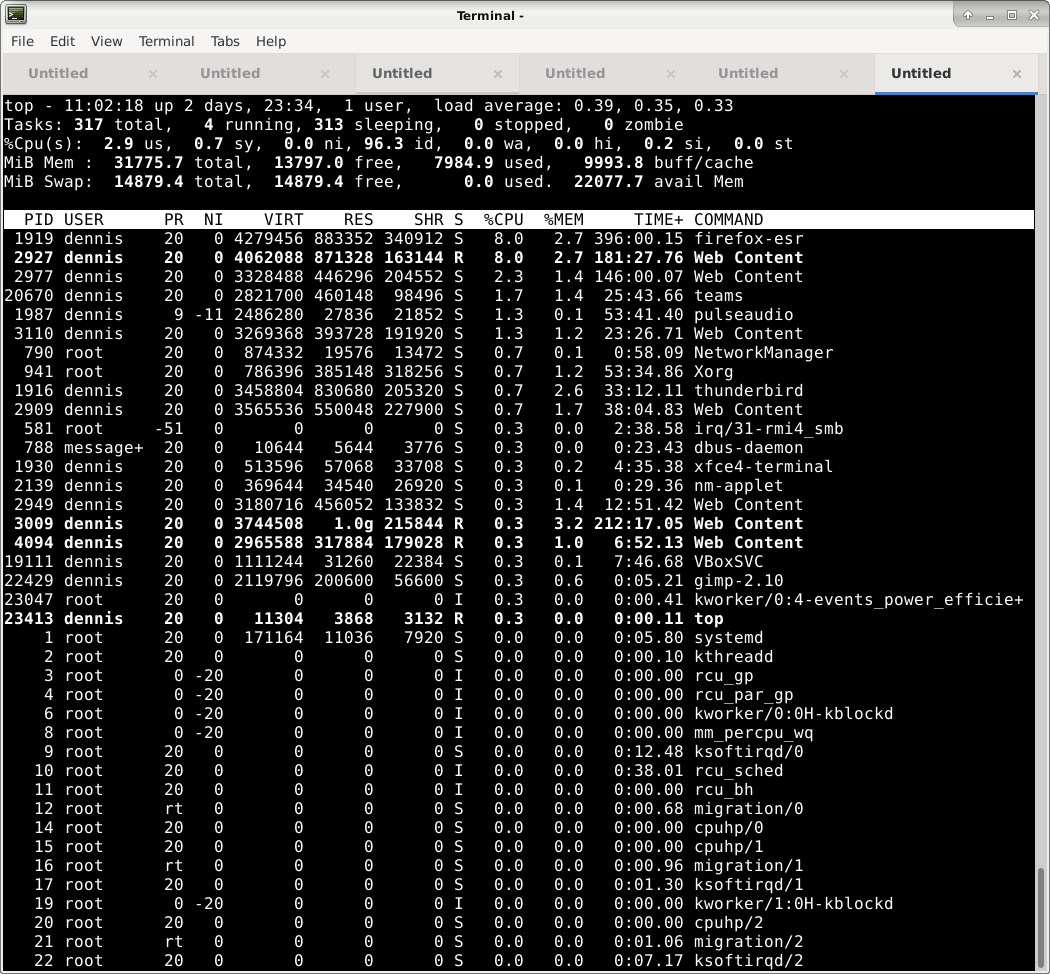
\includegraphics[width=\textwidth]{top}
\centering
\caption{Top}
\label{fig:top}
\end{figure}
Met \texttt{q} verlaten we \texttt{top}.

\texttt{top} geeft je in \'e\'en scherm heel veel informatie over je systeem en welke processen het meeste van je systeem vragen. Standaard sorteert \texttt{top} de processen op processor gebruik. We wie in het lijstje dat \texttt{firefox-esr} 8.0\% CPU gebruikt en 2.7\% van het geheugen. Met M en P (\textbf{let op} hoofdletters), kan je schakelen tussen een overzicht van het meeste processor (P) gebruik of het meeste memory (M) gebruik.

\section{Logging}
Het is belangrijk dat processen informatie kunnen doorgeven aan beheerders van systemen. Een proces moet kunnen melden dat er bijvoorbeeld iets fout is gegaan. Met een grafische applicatie is dat geen probleem, die geeft dan een pop-up op het scherm. Een niet grafische applicatie kan een bericht op de commandline achterlaten, maar een proces dat in de achtergrond draait kan dat niet, die moet zijn meldingen ergens anders kwijt. Dit soort processen schrijven hun meldingen naar een log. Logging is de Engelse term voor vastleggen, opschrijven. Om die logging gestructureerd te doen, en niet elk proces zijn eigen keuze te laten maken, is er een directory genaamd \texttt{/var/log} waarin de log bestanden worden opgeslagen.

Elk proces mag zelf in deze directory schrijven of het mag gebruik maken een de logserver op een Linux systeem. Door gebruik te maken van de logserver worden logberichten op een gestandaardiseerde manier opgeslagen op het systeem.

\subsection{syslog}
Het proces dat op de achtergrond draait en dat verantwoordelijk is voor het schrijven van de verschillende logbestanden heet syslog\index{syslog}, een afkorting van system logging. Het gebruik van syslog heeft als groot voordeel dat niet elke software ontwikkelaar alle code hoeft te schrijven om logbestanden te schrijven, hij hoeft alleen maar te weten hoe hij data moet aanlever bij de syslog server. Voor de systeembeheerder is het makkelijk omdat hij niet elk programma hoeft te vertellen waar deze zijn meldingen weg moet schrijven, die hoeft alleen maar de syslog-server te beheren en het laatste voordeel is dat de output van syslog altijd dezelfde is, dus de logbestanden worden nog makkelijker leesbaar ook.

Vele Linux distributies gebruiken rsyslog\index{rsyslog} als hun syslog server. De belangrijkste logbestanden in de \texttt{/var/log} die beheerd worden door de syslog server zijn:
\begin{description}
\item[\texttt{messages}] Alle logs
\item[\texttt{mail} (SuSE) \texttt{maillog} (RedHat) of \texttt{mail.log} (Debian)] Mail logging
\item[\texttt{mail.info}] Mail info messages
\item[\texttt{mail.warn}] Mail warning messages
\item[\texttt{mail.err}] Mail error messages
\item[\texttt{daemon.log} (Debian)] Berichten van Daemons
\item[\texttt{auth.log} (Debian) of \texttt{secure} (RedHat)] Authenticatie gerelateerde berichten
\end{description}

\subsection{kernel berichten}
De kernel wil ons soms ook wat berichten overbrengen. Zeker tijdens het opstarten van het systeem produceert de kernel vele berichten. De Linux kernel gebruikt een ringbuffer voor deze berichten. Een ringbuffer is een FIFO, First In, First Out, buffer, wat betekend dat berichten in de buffer worden opgeslagen tot de buffer vol is, nieuwere berichten drukken dan de oudste berichten uit de buffer. De standaard buffer grote is 

\texttt{dmesg}\index{dmesg}\index{commando!dmesg} is het commando om deze berichten uit te kunnen lezen. De bootberichten zijn zo belangrijk dat de meeste Linux distributes de ringbuffer na het opstarten leeglezen en deze opslaan als \texttt{/var/log/boot.log} of \texttt{/var/log/boot}. Want ook na het opstarten blijft de kernel naar deze ringbuffer schrijven en nieuwere berichten drukken dan uiteindelijk de berichten die gegenereerd zijn tijdens het opstarten uit de buffer.

Een belangrijke optie voor \texttt{dmesg} is de \texttt{-T} optie. De standaard timestamp in de \texttt{dmesg} output is niet lekker leesbaar, met \texttt{-T} krijgen een output die wel goed leest:
\begin{lstlisting}[language=bash]
$ sudo dmesg -T
[Wed Mar 17 12:41:28 2021] CPU2: Package temperature/speed normal
[Wed Mar 17 12:41:28 2021] CPU1: Core temperature/speed normal
[Wed Mar 17 12:41:28 2021] CPU5: Package temperature/speed normal
[Wed Mar 17 12:41:28 2021] CPU4: Package temperature/speed normal
[Wed Mar 17 12:41:28 2021] CPU7: Package temperature/speed normal
[Wed Mar 17 12:41:28 2021] CPU6: Package temperature/speed normal
[Wed Mar 17 12:41:28 2021] CPU0: Core temperature/speed normal
[Wed Mar 17 12:41:28 2021] CPU3: Package temperature/speed normal
[Wed Mar 17 12:41:28 2021] CPU1: Package temperature/speed normal
[Wed Mar 17 12:41:28 2021] CPU0: Package temperature/speed normal
\end{lstlisting}


% Requires: lsblk
% Provides: mount, umount
\chapter{Mounten van lokale bestandssystemen}
Wat je zal zijn opgevallen als je een Windows-gebruiker bent is dat Linux geen drive letters heeft. In Linux is het hele systeem \'e\'en groot file system waarbij de verschillende disks of partities gemount worden op een directory in het file system.
\begin{lstlisting}[language=bash]
$ lsblk
NAME   MAJ:MIN RM   SIZE RO TYPE MOUNTPOINT
sda      8:0    0 931.5G  0 disk 
|-sda1   8:1    0 931.5G  0 part /home/dennis
sdb      8:16   1  59.8G  0 disk 
|-sdb1   8:17   1  58.8G  0 part /
|-sdb2   8:18   1     1K  0 part 
|_sdb5   8:21   1   976M  0 part [SWAP]
\end{lstlisting}


\section{Mounten van disks}
Een disk of partitie op een disk wordt gemount op het bestandssysteem. Om dit duidelijk te maken moeten we wat dieper in
het systeem duiken en een paar dingen doen die we pas later in dit boek uitleggen. Dus type nauwkeurig het volgende
commando over:

\begin{lstlisting}[language=bash]
$ mount | grep ' / '
\end{lstlisting}

Voor en achter de / staat een enkele spatie. Dit geeft iets terug als:
\begin{lstlisting}[language=bash]
/dev/sda1 on / type ext4 (rw,relatime,errors=remount-ro)
\end{lstlisting}

Wat dit betekent is dat de eerste partitie op de harddisk die het systeem kent als sda gekoppeld (gemount) is op /.
USB-disks kunnen op dezelfde manier gekoppeld worden aan het systeem. De directory die daarvoor gereserveerd is is
/media/. In de /media/ directory zijn er directories per gebruiker waar gebruikers hun USB-disks kunnen mounten. Later
zullen we hier uitgebreider op terug komen.

/mnt is de directorie die van oudsher aanwezig is om lokaal media op te mounten en zou nu alleen nog door de beheerder
gebruikt moeten worden voor het tijdelijk mounten van disks.


\chapter{Netwerk configuratie}

\chapter{Software installeren}

\chapter{Programmeertalen}
Van oudsher werden Unix systemen veel gebruikt door programmeurs. Er zijn dan ook veel talen ontwikkeld en overgezet naar Linux. Natuur is er een C-compiler. De meest gebruikte is die uit het GNU project die de GNU Compiler Collection (GCC) heet omdat hij naast \index{C}C ook compilers bevat voor \index{C++}C++, \index{Objective-C}Objective-C, \index{Fortran}Fortran, \index{Ada}Ada, \index{Go}Go en \index{D}D.

Ook voor scripting talen zijn er veel \foreignlanguage{english}{interpreters} aanwezig zoals voor PHP, Perl, Python en Java.

Daarnaast is er via verschillende kanalen nog veel meer te installeren.

In het document Linux Introductie (ook beschikbaar via https://github.com/DennisLeeuw/Linux) staat beschreven hoe je van C-source code naar een vorm komt die de CPU begrijpt. Dat proces heet compileren. Je gebruikt een compiler om bron-code om te zetten naar binaire code.

Er is nog een andere manier om een programma te draaien op je computer. Je kan ook de broncode omzetten naar binaire code via een runtime engine. Programmeertalen die hiervan gebruik maken heten scripting talen.

Het belangrijkste verschil tussen de twee vormen is de manier waarop een applicatie verspreid wordt. Als je de broncode compileert en er een binairbestand van maakt dan kan je alleen het binaire bestand delen en iedereen met dezelfde OS-versie en hardware kan jouw software dan gebruiken. Dit is wat bijvoorbeeld Apple en Microsoft doen en hoe veel van ook de Linux software verspreid wordt via de repositories. Als je software een script is dan is de verspreiding per definitie als broncode. Een shell-script, JavaScript, PHP of Python wordt bijna altijd als broncode verspreid en een runtime engine wordt gebruikt om het script te starten op de computer.

Scripting had de naam om traag te zijn, maar dat is bij moderne scripting talen zoals Python inmiddels bijna niet meer het geval.


\section{C}
\section{C++}
\section{Perl}
\section{PHP}
\section{Python}
\section{Bash}

\chapter{Shell scripting}\index{Shell scripting}
De meeste besturingssystemen kennen een vorm van scripting. Een scripting taal is een programmeertaal die niet gecompileerd hoeft te worden voordat hij uitgevoerd kan worden. De vertaling naar machinecode vindt plaats op het moment dat het script wordt uitgevoerd. Voor de uitvoer van het script is daarom altijd een interpreter (vertaler) nodig die het script vertaalt naar iets dat de computer snapt.

Er zijn verschillende soorten scripting talen met de daarbij behorende interpreters. Voor Linux systemen zijn de belangrijkste:
\begin{itemize}
\item Shell scripting (bash of sh)
\item Perl
\item PHP
\item Python
\item Java
\end{itemize}

Naast een command interpreter is de shell\index{shell} op elk Linux-systemen ook een interpreter van een scripting taal, de zogenaamde shell-scripts\index{shell-script}. Op Linux systemen is de standaard shell \texttt{bash}\index{bash}\index{commando!bash} en op Mac OS X aanwezig, dus als je programma's kan schrijven die de shell begrijpt kan je ze op veel systemen toepassen. In de meest simpele vorm is een shell-script een lijstje met commando's. Door het script op te starten worden de commando's \'e\'en voor \'e\'en opgestart, maar er is veel meer mogelijk. In dit hoofdstuk ga je leren hoe je shell-scripts schrijft.

\section{Waarom scripting?}
De kracht van shell scripts is dat je de commando's die je op de command line gebruikt direct kunt toepassen in de software die je schrijft. Misschien kunnen we zelfs stellen dat een shell script een lijstje is van commando's die voor later gebruik in de juiste volgorde in het script zijn geplaatst. De vraag is natuurlijk wel, waarom zouden we dat willen?

De belangrijkste reden is dat als er herhaalde handelingen gedaan moeten worden dat de computer dat nauwkeuriger kan dan een mens. Als je eenmaal een script hebt geschreven dat werkt kan je het meerdere keren achter elkaar laten uitvoeren zonder dat er typefouten ontstaan, terwijl typefouten bij mens de meest voorkomende fout is bij het uitvoeren van een commando.

Als het complexe handelingen zijn is het helemaal handig om dit vast te leggen in een script zodat je zeker weet dat je geen stappen over zal slaan.

En als laatste zijn er soms taken die herhaald uitgevoerd moeten worden op vaste dagen of tijden. Denk hierbij aan bijvoorbeeld backups. Het Linux systeem heeft hiervoor een stukje software dat \texttt{cron}\index{cron}\index{commando!cron} heet en dat op gezette tijden een commando kan uitvoeren. Door verschillende commando's in een script te plaatsen en \texttt{cron} te vertellen het script uit te voeren kunnen er verschillende handelingen in een keer uitgevoerd worden.

\section{Hello World - een eerste script}
We gaan een bestand maken met de naam texttt{hello\_world.sh}\index{hello\_world.sh}. Het is een goeie gewoonte om een bestandsnaam te eindigen met een extensie die weergeeft wat voor type bestand het is. Dit is voor Linux niet noodzakelijk, maar voor ons gebruikers is het handig om te weten dat we te maken hebben met een shell-script en dus eindigen we de bestandsnaam met .sh.

Om structuur in ons werk te houden maken we een directory scripts aan in onze home directoy.
\begin{lstlisting}[language=bash]
$ cd ~
$ mkdir scripts
$ cd scripts
\end{lstlisting}
Maak met \texttt{vi} het bestand hello\_world.sh aan en plaats in het bestand de volgende tekst:
\begin{lstlisting}[language=bash]
echo "Hello world!"
exit 0
\end{lstlisting}
Sluit \texttt{vi} af. We hebben nu een bestand met 2 commando's. Regel 1 zegt beeld Hello World! op het scherm af en regel 2 zegt verlaat dit script. Linux leest echter geen extensies om te bepalen wat het moet doen, maar het leest de eerste twee characters van een bestand om te bepalen wat er met een bestand gedaan moet worden. Deze eerste twee characters van een bestand heten het magic number\index{magic number}.

Het \texttt{file}\index{file}\index{commando!file} commando kan gebruikt worden om het magic nummer van een bestand te lezen en weer te geven wat voor soort bestand het is.
\begin{lstlisting}[language=bash]
$ file hello_world.sh
hello_world.sh: ASCII text
\end{lstlisting}
We zien dat Linux nog denkt dat het om een text bestand gaat. Het ziet het niet als een shell script. Voeg nu boven de \texttt{echo} regel een regel toe zodat je script er zo uit komt te zien:
\begin{lstlisting}[language=bash]
#!/bin/bash
echo "Hello world!"
exit 0
\end{lstlisting}
Als je de editor verlaten hebt en weer een \texttt{file} doet van hello\_world.sh dan zal je zien dat Linux nu weet dat het om een shell-script gaat.

Voor een script dat ge\"interpreteerd moet worden door een interpreter, dat kan een shell zijn, zijn de 2-character codes de she-bang\index{she-bang}: \#! of hexadecimaal 0x23 0x21. Achter de she-bang komt de interpreter die het script moet interpreteren. Als de shell deze character reeks tegen komt zal het de rest van de regel lezen om te bepalen aan welke interpreter (shell) het het script moet voeren. In ons voorbeeld wordt het script gegeven aan het programma /bin/bash en deze zal de twee opgegeven commando's uitvoeren.

Eerst wordt door echo \texttt{Hello world!} op het scherm gezet en daarna sluit het script af. Het \texttt{exit}\index{exit}\index{commando!exit}\index{Shell scripting!exit} commando is niet noodzakelijk, als de shell geen commando's meer tegen komt zal het automatisch afsluiten. Het voordeel van \texttt{exit} is dat je er een exit code aan kan meegeven zodat je kan laten weten dat het script goed (0) of fout (1) ge\"eindigd is. Doe je dit niet dan is de exit code de error-code van het laatst uitgevoerde commando.

Voer het script uit en geef direct daarna het commando
\begin{lstlisting}[language=bash]
$ echo $?
\end{lstlisting}
als je nu de regel met daarop \texttt{exit 0} vervangt door \texttt{exit 1} en dan weer het script draait en het commando
\begin{lstlisting}[language=bash]
$ echo $?
\end{lstlisting}
geeft dan zie welke invloed het exit commando heeft.

\section{Het starten van scripts}\index{Shell scripting!Starten}
Het script kan op twee verschillende manieren opgestart worden. Allereerst kunnen we script rechtstreeks aan de shell geven:
\begin{lstlisting}[language=bash]
$ bash ./hello_world.sh
\end{lstlisting}
De tweede mogelijkheid is dat we het script executable maken en daarna direct uitvoeren. We kunnen een script executable maken voor de eigenaar door het x-bit te zetten voor de user:
\begin{lstlisting}[language=bash]
$ chmod u+x ./hello_world.sh
\end{lstlisting}
Daarna kan de eigenaar het script direct uitvoeren
\begin{lstlisting}[language=bash]
$ ./hello_world.sh
\end{lstlisting}
Bij beide opties is het van belang om het complete pad mee te geven aan het script. In de voorbeelden konden we volstaan met ./ omdat het script in de directory staat waar we al in staan. Maar we zouden ook het volledige pad kunnen opgeven:
\begin{lstlisting}[language=bash]
$ /home/dennis/scripts/hello_world.sh
\end{lstlisting}
We kunnen ook het pad /home/dennis/scripts toevoegen aan onze PATH variabele en er zo voor zorgen dat we nooit meer het pad hoeven op te geven.
\begin{lstlisting}[language=bash]
$ export PATH=$PATH:/home/dennis/scripts
$ hello_world.sh
\end{lstlisting}

\section{Commentaar}\index{Shell scripting!commentaar}
Op het moment dat je een programma schrijft is het meestal volledig duidelijk wat je aan het doen bent en waarom. Als het script complexer wordt is het soms al lastiger en als je er na een jaar naar kijkt heb je soms geen idee meer waarom je het hebt gemaakt en hoe het ook alweer in elkaar zat. Het is daarom goed om uitleg in je script te verwerken. Dit maakt het voor jezelf duidelijker, maar ook als iemand anders iets wil wijzigen aan wat jij gemaakt hebt maakt het het voor die persoon een stuk makkelijker als hij of zij weet wat er waar gebeurd in het script.
Open met vi het hello\_world.sh\index{hello\_world.sh} script en wijzig het zo dat het er zo uit komt te zien:
\begin{lstlisting}[language=bash]
#!/bin/bash
# (c) 2020, Dennis Leeuw
# License: GPL v3
# Versie: 1.0
# Dit script print Hello world! Op het scherm

echo "Hello World!"
# Verlaat het script met error-code 0
exit 0
#END
\end{lstlisting}
Je hebt nu 5 regels commentaar toegevoegd. Het \# symbool geeft dat het commentaar is en dat de interpreter (de shell) er niets mee moet doen. Als je het script opnieuw uitvoert zie je dat er niets gewijzigd is aan de uitvoer.

Vervang aan het commentaar het jaartal 2020 naar het jaartal waarin je nu leeft en verander de naam Dennis Leeuw in je eigen naam.

Het is een goede gewoonte om aan te geven wie een script gemaakt heeft, wat de licentie is en een korte beschrijving te geven van wat het script doet. Je werkt waarschijnlijk niet je leven lang op dezelfde afdeling of waarschijnlijk niet eens bij hetzelfde bedrijf. Beheerders na jou kunnen op deze manier snel zien wie iets gemaakt heeft en wat het script doet.

Ik laat mijn scripts meestal eindigen met \#END zodat ik weet of het script compleet is. Als het script begint met een she-bang en eindigt met \#END dan is het script compleet.

\section{Variabelen}\index{Variabelen, shell scripting}\index{Shell scripting!Variabelen}
Een variabele is een plek om data in op te slaan voor later gebruik. We kunnen ons script aanpassen op de volgende manier om een voorbeeld te geven van het gebruik van een variabele in scripts:
\begin{lstlisting}[language=bash]
#!/bin/bash
# (c) 2020, Dennis Leeuw
# License: GPL v3
# Versie: 1.1
# Dit script print Hello world! Op het scherm

output="Hello world!"
echo $output
# Verlaat het script met error-code 0
exit 0
#END
\end{lstlisting}

We hebben nu een variabele met de naam output toegevoegd en deze variabele hebben we de waarde (data) "Hello world!" gegeven.

Bij het echo-commando\index{echo} gebruiken we de variabele om weer onze vertrouwde uitvoer te krijgen.

Let er op dat bij het declareren (het van een waarde voorzien) van de variabele er geen dollar-teken voor de variabele staat, maar bij het gebruik wel.

De shell heeft ook een aantal ingebouwde variabelen\index{ingebouwde variabelen}\index{builtin variables}\index{variabelen!ingebouwde}. Deze variabelen worden met allemaal hoofdletters geschreven. Om verwarring te voorkomen is het dus handig om je eigen variabelen niet met allemaal hoofdletters te schrijven. De meest gebruikte shell-variabelen in scripts zijn \$USER die de gebuikersnaam bevat, \$HOME die de home-directory bevat en \$PWD die het complete directory pad bevat vanaf de root tot de directory waarin de gebruiker stond toen hij het script startte. Probeer dit script uit:
\begin{lstlisting}[language=bash]
#!/bin/bash
# (c) 2020, Dennis Leeuw
# License: GPL v3
# Versie: 1.1
# Vertelt de gebruiker met welke gebruikersnaam hij of zij ingelogd is, wat
# zijn of haar home-directory is en in welke directory hij of zij nu staat.

echo "Je bent ingelogd als $USER en je home-directory is $HOME"
echo "Je huidige directory is $PWD"

exit 0
#END
\end{lstlisting}

Variabelen worden dus gebruikt om data in op te slaan. Je kan ook de uitvoer van een commando in een variabele stoppen. Op Linux bestaat er het commando \texttt{date}\index{date}\index{commando!date} dat op verschillende manieren informatie over de datum en tijd kan weergeven en waarmee je de datum en tijd op je computer kan zetten. Omdat date zoveel kan lijkt het in eerste instantie ingewikkeld, maar als je er een beetje ervaring mee op doet blijkt het een enorm handige tool te zijn. Tikken we alleen date in op de commandline en daarna enter, dan krijgen we van het systeem de huidge datum en tijd terug en in welke tijdzone we leven. Als we bijvoorbeeld alleen het jaar willen weten waarin we nu leven dan vragen we dat aan date door:
\begin{lstlisting}[language=bash]
date +%Y
\end{lstlisting}
en alleen de maand is:
\begin{lstlisting}[language=bash]
date +%m
\end{lstlisting}
dit is het maandnummer, willen de naam van de maand dan gebruiken we:
\begin{lstlisting}[language=bash]
date +%B
\end{lstlisting}
Meer van deze opties vind je terug in de manual-pagina van texttt{date}. Lees deze door zodat je ook weet hoe je de dag, de uren en de minuten moet weergeven.

Om in een script de uitvoer van \texttt{date} in een variabele te zetten kunnen we het volgende gebruiken:
\begin{lstlisting}[language=bash]
#!/bin/bash
# (c) 2021, Dennis Leeuw
# License: GPL v3
# Versie: 1.0
# Wat is de huidige datum en tijd

start="$(date '+%Y-%m-%d-%H-%M')"

echo ${start}

exit 0
#END
\end{lstlisting}
We hebben nu de uitvoer van het \texttt{date} commando aan een variabele gegeven en deze geprint. Let op de quotes! Als we parameters aan een commando willen voeren die ook een betekenis in de shell hebben, zoals in dit geval het \%-teken, dan moeten we de parameter tussen enkele quotes zetten zodat ze door de shell niet ge\"interpreteerd worden.

De laatste manier om een variabele een waarde te geven is door aan de gebruiker input te vragen, hiervoor bestaat er het \texttt{read}\index{read}\index{commando!read} commando. In een script zou je dat zo kunnen gebruiken:
\begin{lstlisting}[language=bash]
#!/bin/bash
# (c) 2021, Dennis Leeuw
# License: GPL v3
# Versie: 1.0
# Vraag de gebruiker om zijn leeftijd

echo -n "Hallo $USER, hoe oud ben jij? "
read leeftijd

echo "De gebruiker $USER is $leeftijd jaar oud."

exit 0
#END
\end{lstlisting}


\section{if}\index{if}\index{Shell scripting!if}
Je kan een script gebruiken om alle commando's die je op de commandline gebruikt onder elkaar te zetten als een lange lijst. Beter is het als je ook controleert of een commando succesvol is verlopen. Eerder hebben we behandeld dat de exit code van een commando terecht komt in de variabele \$?. Als we een test zouden kunnen doen in een script om te zien of deze variabele 0 is, dus als alles goed is verlopen, dan kunnen we controleren of er commando's fout zijn gegaan.

Er is een commando dat \texttt{test}\index{test}\index{commando!test} heet dat doet wat het zegt, je kan er dingen mee testen, en de uitkomst is waar (true) of nietwaar (false), andere opties zijn er niet. Dit commando gaan we niet direct in een script gebruiken, maar eerst eens op de commandline uitproberen om te zien wat we ermee kunnen.
\begin{lstlisting}[language=bash]
$ touch test_bestand.txt
$ test -f test_bestand.txt
$ echo $?
$ test -f deze_bestaat_niet
$ echo $?
$ file -s test_bestand.txt
$ echo $?
\end{lstlisting}
Lees de manual-page van \texttt{test} eens door en zoek uit wat de \texttt{-s} optie betekent.

Het \texttt{test} commando kan ook gebruikt worden om waarden met elkaar te vergelijken. \texttt{test} maakt daarin in onderscheid tussen strings en integers (getallen).
\begin{lstlisting}[language=bash]
$ test "Aap" = "Aap"; echo $?
$ test "Aap" = "Aapje"; echo $?
$ test "01" = "1"; echo $?
$ test "01" -eq "1"; echo $?
\end{lstlisting}
Zoals je gezien zult hebben test de = op het gelijk zijn van strings en -eq op het gelijk zijn van integers, waarbij 01 gelijk is aan 1.

Strings kan je vergelijken met = om te zien of ze aan elkaar gelijk zijn en met != om te zien of ze niet aan elkaar gelijk zijn.

Met integers kan je nog veel meer vergelijkingen maken:
\begin{description}
	\item[-eq] Controlleer of integers gelijk zijn (equal)
	\item[-ne] Controlleer of integers ongelijk zijn (not equal)
	\item[-gt] Controlleer of eerste integer groter is dan de tweede (greater then)
	\item[-ge] Controlleer of de eerste integer groter of gelijk is aan de tweede (greater or equal)
	\item[-lt] Controlleer of eerste integer kleiner is dan de tweede (less then)
	\item[-le] Controlleer of de eerste integer kleiner of gelijk is aan de tweede (less or equal)
\end{description}
In de manual pagina vind je nog veel meer mogelijkheden waarop je kan testen met \texttt{test}, maar voor ons zijn dit de belangrijkste opties. We gaan de opgedane kennis toepassen in shell-scripts.

Het eerste script dat we gaan maken is een script dat een \texttt{ping}\index{Shell scripting!ping} doet naar een IP-adres en dat test of de ping goed verlopen is:
\begin{lstlisting}[language=bash]
#!/bin/bash
# (c) 2021, Dennis Leeuw
# ping een host en kijk of dat succesvol is verlopen

ip="192.168.10.42"

ping -c1 ${ip} 2>/dev/null 1>/dev/null
if [ $? -ne 0 ]
	then
	echo "Het ${ip} is niet aanwezig op het netwerk"
fi

exit 0
#END
\end{lstlisting}
We voeren hier het \texttt{ping}\index{ping}\index{commando!ping} commando uit en sturen de error en andere berichten naar \texttt{/dev/null}. Als de return code in \$? niet 0 is, dus 1 of hoger is, dan heeft onze ping geen antwoord gekregen en vertellen we dat aan de gebruiker.

Het zal opgevallen zijn dat we bij de \texttt{if} twee bijzondere tekens hebben neergezet [ en ]. Deze tekens betekenen dat er een test gedaan moet worden. We hadden de regel ook zo kunnen schrijven:
\begin{lstlisting}[language=bash]
if test $? -ne 0
\end{lstlisting}
Het is echter een goede gewoonte om in scripts de blokhaken, [ en ], te gebruiken.

Stel dat we ook aan de gebruiker willen laten weten als het wel goed gegaan is. Dus in alle andere gevallen, dat kunnen we doen met \texttt{else}\index{else}\index{Shell scripting!else}:
\begin{lstlisting}[language=bash]
#!/bin/bash
# (c) 2021, Dennis Leeuw
# ping een host en kijk of dat succesvol is verlopen

ip="192.168.10.42"

ping -c1 ${ip} 2>/dev/null 1>/dev/null
if [ $? -ne 0 ]
	then
	echo "Het ${ip} is niet aanwezig op het netwerk"
	else
	echo "Het ${ip} is wel op het netwerk aangetroffen"
fi

exit 0
#END
\end{lstlisting}
Probeer dit script ook eens met een ander IP adres, bijvoorbeeld 127.0.0.1.

De \texttt{if, then, else} kent in bash nog een toevoeging namelijk de \texttt{elif}. De \texttt{elif} is een samentrekking van \texttt{else} en \texttt{if} en kan gebruikt worden om meerdere tests na elkaar te doen. Bijvoorbeeld:
\begin{lstlisting}[language=bash]
#!/bin/bash
# (c) 2021, Dennis Leeuw
# test een getal

getal=15

if [ ${getal} -le 10 ]; then
	echo "Getal is kleiner of gelijk aan 10"
elif [ ${getal} -ge 20 ]; then
	echo "Getal is groter of gelijk aan 20"
else
	echo "Getal ligt tussen 10 en 20"
fi
\end{lstlisting}
Neem dit script over en varieer de waarde van de variabele \texttt{getal}, zodat het het script een keer door de \texttt{if} loopt, een keer door de \texttt{elif} en een keer door de \texttt{else}.

\subsection{Opdracht: Werken met if}
\begin{enumerate}
\item Maak een script dat aan de gebruiker een getal vraagt en geef weer of het getal kleiner of gelijk is aan 10, groter is dan 10 en kleiner of gelijk is aan 20, groter is dan 20 en kleiner of gelijk is aan 30 of groter is dan 30.
	
\item Maak een script dat test of een bestand leeg is. Als het bestand leeg is moet het verwijderd worden.

\item Maak een script dat aan de gebruiker om twee bestandsnamen vraagt. Test of de bestanden bestaan en kijk dan wel bestand nieuwer is. Laat aan de gebruiker weten welk bestand het nieuwste is. Tips: lees de manual-pagina van \texttt{test} en om te testen lees de manual-pagina van \texttt{touch}.
\end{enumerate}

\section{for}\index{for}\index{Shell scripting!for}
Om een handeling een bepaald aantal keren uit te voeren kunnen we gebruik maken van \texttt{for}. Met behulp van \texttt{for} kunnen we een loop doorlopen. Het \texttt{for} commando heeft twee hulpcommando's nodig, namelijk \texttt{do}\index{Shell scripting!do} en \texttt{done}\index{Shell scripting!done}. Na het \texttt{for} commando komt de conditie waaraan we moeten voldoen en tussen \texttt{do} en \texttt{done} staat de loop die doorlopen wordt. Laten we beginnen met een voorbeeld:
\begin{lstlisting}[language=bash]
#!/bin/bash
# (C) 2021 Dennis Leeuw
# License: GPLv3
# Tel van 1 tot 10

list="1 2 3 4 5 6 7 8 9 10"

for i in ${list}
do
	echo $i
done

#END
\end{lstlisting}
In dit script wordt op basis van een lijstje getallen elk getal \'e\'en voor \'e\'en aan de variabele i toegekend, dit is de conditie waaraan de \texttt{for} loop moet voldoen. Zolang er nog een parameter (getal) is wordt de loop tussen \texttt{do} en \texttt{done} doorlopen.

Tussen de commando's die het begin (\texttt{do}) en het einde van de loop (\texttt{done}) aangeven staan de commando's die in de loop uitgevoerd moeten worden. In ons geval is dat maar \'e\'en commando namelijke echo \$i.

Wat je misschien opgevallen is is dat de shell automatische weet dat hij de getallen 1 tot en met 10 als losse waarden moet beschouwen en deze aan de variabele i moet toekennen. We zouden het script kunnen herschrijven met quotes en zien wat er dan gebeurd:
\begin{lstlisting}[language=bash]
#!/bin/bash
# (C) 2021 Dennis Leeuw
# License: GPLv3
# Tel van 1 tot 10

list="'1 2' 3 4 '5 6' 7 8 '9 10'"

for i in ${list}
do
	echo $i
done

#END
\end{lstlisting}
Neem dit script over, let goed op de enkele quotes, en start het script. Ook hier geldt dus wat de enkele quotes (ticks) ervoor zorgen dat spaties niet meer gebruikt worden als scheidingsteken.

De vraag die hopelijk nu ontstaan is is waarom gebruikt de shell een spatie als scheidingsteken? Dat komt omdat de shell een interne variabele kent die \texttt{IFS}\index{IFS}\index{Internal Field Separator} heet en dat staat voor Internal Field Separator (interne veld scheider). Deze variabele bepaalt hoe de shell met velden omgaat. Standaard gebruikt de shell, spaties, tabs en de nieuwe regel (enter) als scheidingstekens. Ik kan het bovenstaande script dan ook herschrijven met nieuwe regels zonder dat de werking veranderd:
\begin{lstlisting}[language=bash]
#!/bin/bash
# (C) 2021 Dennis Leeuw
# License: GPLv3
# Tel van 1 tot 10

list="1
2
3 4
5
6 7
8
9 10"

for i in ${list}
do
	echo $i
done

#END
\end{lstlisting}
Het is minder goed leesbaar, maar voor de werking maakt het niet uit. We kunnen de IFS ook aanpassen. We maken nu een nieuw script waarin we het scheidingsteken (\texttt{IFS}) naar een newline (nieuwe regel) zetten en de \texttt{list} variabele ophakken in twee stukken:
\begin{lstlisting}[language=bash]
#!/bin/bash
# (C) 2021 Dennis Leeuw
# License: GPLv3
# Tel van 1 tot 10

# Set the IFS variable to newline
IFS=$'\n'

list="1 2 3 4 5
6 7 8 9 10"

# Count from 1 to 10 ... or not
for i in ${list}
do
	echo $i
done

#END
\end{lstlisting}
De uitvoer zal er dan zo uitzien
\begin{lstlisting}[language=bash]
$ ./script_for_IFS.sh 
1 2 3 4 5
6 7 8 9 10
\end{lstlisting}
Alleen de newline scheidt dan nog de delen en de spaties worden niet meer gezien als scheidingsteken.

Je kan de \texttt{IFS} naar elk willekeurig character zetten:
\begin{lstlisting}[language=bash]
#!/bin/bash

IFS="n"
zin="Dit is een zin en daarin komt vaak de n voor"
for i in $zin
do
	echo $i
done
\end{lstlisting}
De n is nu het scheidingsteken geworden en dat betekent dat de uitvoer van dit script er zo uit komt te zien:
\begin{lstlisting}[language=bash]
$ ./testscriptIFS.sh
Dit is ee
 zi
 e
 daari
 komt vaak de
 voor
\end{lstlisting}
Je ziet dat alle n-en zijn verdwenen en dat de zin is opgehakt op de plek waar de n stond.

\subsection{Opdracht: Werken met for}
Voor elke nieuwe gebruiker willen we vast een aantal directories maken binnen het bedrijf waarin we werken. Als de directory al aangemaakt is moet die niet gemaakt worden en als hij nog niet bestaat moet hij wel aangemaakt worden. De input van het script moet de naam van de gebruiker zijn. Maak gebruik van \texttt{for} om in een loop de directories aan te maken. De directory-tree die aangemaakt moet worden is:
\begin{itemize}
\item Documenten/Werkoverleg
\item Documenten/Werkoverleg/Verslagen
\item Documenten/Werkoverleg/Actiepunten
\item Documenten/Handleidingen
\item Documenten/Klanten
\item Documenten/Klanten/Systeem\_documentatie
\item Documenten/Servers/Systeem\_documentatie
\item Documenten/Servers/Inkoop\_documenten
\item Documenten/Servers/Handleidingen
\item Scripts
\end{itemize}

\section{while}\index{while}\index{Shell scripting!while}
Om door een lijst met elementen te lopen tot een bepaalde conditie is bereikt gebruiken we \texttt{while}. \texttt{while} kent hetzelfde begin en eind van de loop als \texttt{for}, namelijk \texttt{do} en \texttt{done}. Een voorbeeld van het gebruik van \texttt{while} zou kunnen zijn:
\begin{lstlisting}[language=bash]
#!/bin/bash
# (C) 2021 Dennis Leeuw
# While voorbeeld

i=1
while [ $i -le 10 ]
do
	echo $i
	i=$(($i+1))
done

#END
\end{lstlisting}
Dit script lijkt erg op de \texttt{for}-loop uit de vorige paragraaf. We vertellen hier dat de variabele \texttt{i} 1 is en vragen aan \texttt{while} om de loop te doorlopen zolang \texttt{i} kleiner of gelijk is aan 10. Om te zorgen dat \texttt{i} bij elke keer dat de loop doorlopen wordt 1 hoger wordt, moeten we bij \texttt{i} 1 optellen. Rekenen in de shell doen we door gebruikt te maken van dubbele haken, de uitkomst van de berekening zetten we weer in \texttt{i} waardoor \texttt{i} 1 hoger wordt. Deze manier van rekenen kan je ook op de commandline gebruiken, daar heb je niet alleen de shell voor nodig.

In de opgave uit de vorige paragraaf heb je een script gemaakt dat bepaalde directories aanmaakt op basis van een gebruikersnaam die wordt ingegeven door de gebruiker. Van de Linux commando's ben je inmiddels gewend dat je met opties waarden kan meegeven. Het zou natuurlijk heel mooi zijn als je die gebruikersnaam ook met een optie mee zou kunnen geven aan een script. En dat kan ook. In scripting heten parameters of opties die je meegeeft bij het opstarten van een script positional parameters\index{positional parameters}\index{Shell scripting!positional parameters}. Deze positional parameters hebben nummers en lopen van 0 tot het getal van de laatste parameter. Positional parameter 0 is altijd de naam van het script inclusief het pad waarmee het is opgestart.
\begin{lstlisting}[language=bash]
#!/bin/bash
# (C) 2021 Dennis Leeuw
# Positional parameters

echo "Dit script is opgestart als: $0"

echo "Parameter 1 is: $1"
echo "Parameter 2 is: $2"
echo "Parameter 3 is: $3"

#END
\end{lstlisting}
als we dit script opstarten met wat parameters kan krijgen we dit:
\begin{lstlisting}[language=bash]
$ ./scriptWhilePosPar.sh aap noot mies
Dit script is opgestart als: ./scriptWhilePosPar.sh
Parameter 1 is: aap
Parameter 2 is: noot
Parameter 3 is: mies
\end{lstlisting}
De eerste optie is in \$1 terecht gekomen, de tweede in \$2 enzovoort.

In dit script is het natuurlijk onhandig dat we voor elke positionele parameter een regel schrijven. Het zou makkelijker zijn als we de positionele paramaters \'e\'en voor \'e\'en zouden kunnen doorlopen. Een commando dat handig is bij het gebruik van positional parameters is \texttt{shift}\index{shift}\index{Shell scripting!shift}. Met \texttt{shift} schuiven we de positional parameters een positie op. De waarde van parameter 3 wordt de waarde van parameter 2, de waarde van parameter 2 wordt de waarde van parameter 1 en de waarde van parameter 1 wordt weggegooid. Dit kunnen we gebruiken om zo door de hele lijst aan positional parameters te lopen.

\begin{lstlisting}[language=bash]
#!/bin/bash
# (C) 2021 Dennis Leeuw
# While voorbeeld 2

echo "Dit script is opgestart als: $0"

i=1
while [ "$1" != "" ]
do
	echo "Parameter $i is: $1"
	shift
	i=$(($i+1))
done

#END
\end{lstlisting}
De uitvoer van dit script is hetzelfde als het vorige, maar we hoeven nu niet meer voor elke parameter een regel te maken, plus dat het ook niet meer uitmaakt hoeveel parameters we meegeven. Met het gebruik van \texttt{shift} en \texttt{while} kunnen we de positionele parameters doorlopen opzoek naar opties die meegegeven zijn aan een script.

\subsection{Opdracht: Werken met While}
Maak een script dat werkt met de volgende 3 opties:
\begin{itemize}
	\item Als er een optie -u meegegeven wordt, dan is wat er achter -u komt een gebruikersnaam
	\item Als er een optie -d meegegeven wordt, dan is wat er achter -d komt een directory
	\item Als er een optie -h gegegeven wordt dan wordt er een beschrijving van het script weergegeven en stopt het script.
\end{itemize}
De opties -u en -d mogen in willekeurig volgorde aan het script meegegeven worden. Laat als resultaat op het scherm zien welke gebruikersnaam en welke directory als input gegeven zijn.

\section{Opdracht: Gemiddelde cijfer van een student}
In het klas.csv bestand staan de leerlingen van meester Tom. De meeste leerlingen hebben 5 toetsen gemaakt, maar een enkeling door ziekt minder. Meester Tom wil het gemiddelde cijfer weten per student, zodat hij het eindcijfer met de klas kan delen. Voor degene die een toets gemist hebben wordt het cijfer niet door 5 gedeeld maar door het aantal toetsen dat ze echt gemaakt hebben.


%%%%%%%%%%%%%%%%%%%%%
%%% Index and End %%%
%%%%%%%%%%%%%%%%%%%%%
\backmatter
\printindex
\end{document}

%%% Last line %%%
